\documentclass[12pt]{article}
\usepackage{pictex,amsmath,amssymb,amsbsy,amsfonts}
\usepackage{graphics,graphicx}
\usepackage{mathabx}

\setlength{\voffset}{-0.25in}
\setlength{\headsep}{+0.6in}
\setlength{\parskip}{1em}
\setlength{\parindent}{0em}

\def\vu{\mathbf{u}}
\def\vv{\mathbf{v}}
\def\vb{\mathbf{b}}
\def\vs{\mathbf{s}}
\def\vw{\mathbf{w}}

\usepackage{xcolor}
\usepackage{titlesec}
\usepackage{mdframed}
\usepackage[utf8]{vietnam}



\usepackage{listings}
\definecolor{vgreen}{RGB}{104,180,104}
\definecolor{vblue}{RGB}{49,49,255}
\definecolor{vorange}{RGB}{255,143,102}

\lstdefinestyle{verilog-style}
{
    language=Verilog,
    basicstyle=\small\ttfamily,
    keywordstyle=\color{vblue},
    identifierstyle=\color{black},
    commentstyle=\color{vgreen},
    numbers=left,
    numberstyle=\tiny\color{black},
    numbersep=10pt,
    tabsize=8,
    moredelim=*[s][\colorIndex]{[}{]},
    literate=*{:}{:}1
}

\makeatletter
\newcommand*\@lbracket{[}
\newcommand*\@rbracket{]}
\newcommand*\@colon{:}
\newcommand*\colorIndex{%
    \edef\@temp{\the\lst@token}%
    \ifx\@temp\@lbracket \color{black}%
    \else\ifx\@temp\@rbracket \color{black}%
    \else\ifx\@temp\@colon \color{black}%
    \else \color{vorange}%
    \fi\fi\fi
}
\makeatother

\usepackage{trace}


\newmdenv[linecolor=blue,skipabove=\topsep,skipbelow=\topsep,leftmargin=5pt,rightmargin=-5pt,innerleftmargin=5pt,innerrightmargin=5pt]{mybox}

\begin{document}
\begin{center}
\textbf{DIGITAL SYSTEM}
\end{center}
\section{Digital and Analog Systems}
\begin{itemize}
	\item \textbf{Digital System} is a combination of devices that manipulate values represented in digital form.
	\item \textbf{Analog System} is a combination of devices that manipulate values represented in analog form.
\end{itemize}
\subsection*{Analog-to-digital conversion(ADC) and digital-to-analog conversion(DAC) complicate circuitry}
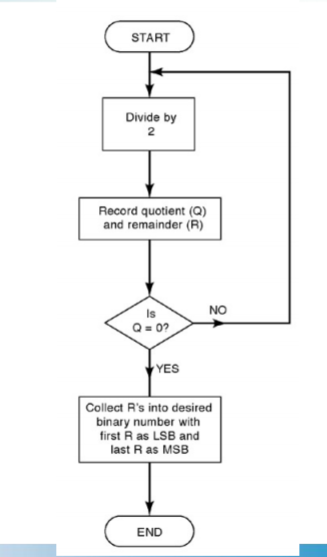
\includegraphics[scale=0.75]{hinh}
\section{Digital Number Systems}
-  Number system differ in the number of symbols they use\\
\begin{itemize}
	\item  Decimal - 10 symbols (base 10)
	\item  Hexadecimal - 16 symbols (base 16)
	\item  Octal - 8 symbols (base 8)
	\item  Binary - 2 symbols (base 2)
\end{itemize}
\section{Conversion}
\subsection*{Binary to Decimal Conversion}
1 \: 0 \: 0 \: 1 \: 0 \: $1_2$ \\
5 \: 4 \: 3 \: 2 \: 1  \:  0
We consider that:\\
$(100101)_2 = 1 \times 2^5 + 0 \times 2^4 + 0 \times 2^3 + 1 \times 2^2 + 0 \times 2^1 + 1 \times 2^0 = (37)_{10}$
\subsection*{Decimal to Binary Conversion}
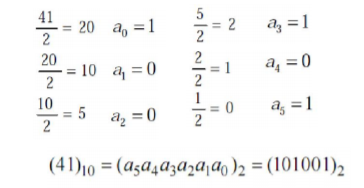
\includegraphics{hinh2}\\
\textbf{Flow chart:}\\
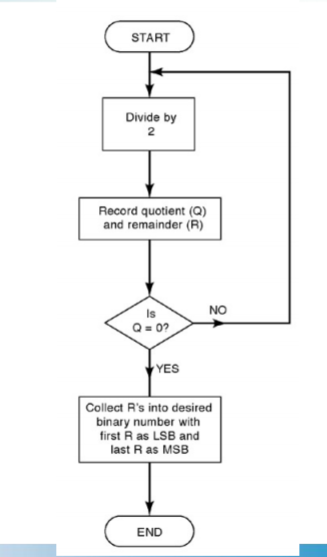
\includegraphics{hinh}
\subsection*{Convert from Hexadecimal to Decimal}
- Convert from Hexadecimal to decimal by multiplying each hex digit by its positional weight\\
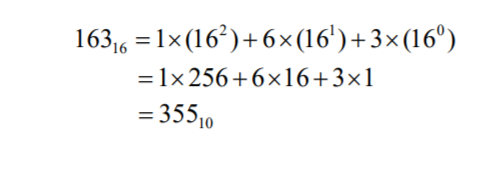
\includegraphics{hinh3}
\subsection*{Hexadecimal to Decimal Conversion}
- Convert form Hexadecimal to Decimal by deviding the decimal number by 16\\
Same method to convertion from binary to decimal\\
\subsection*{Hexadecimal to Binary Conversion}
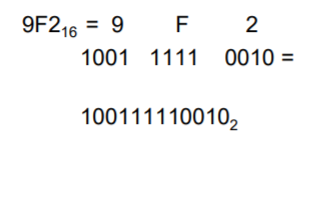
\includegraphics{hinh4}
\subsection*{Binary to Hexadecimal Convertion}
- To convert Binary to Hexadecimal, first we should group bits in four, then we convert each group to hexadecimal.\\
Ex:\\
$1110100110_2 = 0011 \: 1010 \: 0110$ \\
 = 3 \: A \: 6 \\
 = $3A6_{16}$
\section{BCD}
\begin{itemize}
	\item \textbf{Binary Coded Decimal} (BCD) is a another way to present decimal numbers in binary form.
 	\item BCD is widely uses and combines features of both decimal and binary systems.
 	\item Each digit is converted to a binary equivalent.
\begin{table}[h!]
\begin{center}
	\caption{BCD Table}
	\begin{tabular}{|c|c|}
	\hline
	\textbf{Decimal} & \textbf{BCD} \\
	\hline
	0 & 0000\\
	\hline
	1 & 0001\\
	\hline
	2 & 0010\\
	\hline
	3 & 0011\\
	\hline
	4 & 0100\\
	\hline
	5 & 0101\\
	\hline
	6 & 0110\\
	\hline
	7 & 0111\\
	\hline
	8 & 1000\\
	\hline
	9 & 1001\\
	\hline
	\end{tabular}
\end{center}
\end{table}
	\item To convert the number $874_{10}$ to BCD: \\
	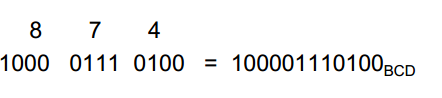
\includegraphics{hinh5}
	\item Each decimal digit is represented using 4 bits
	\item Each 4-bit group can never be greater than 9.
	\item Reverse the process to convert BCD to decimal.
\end{itemize}
\section{Combinational Logic circuit and Sequential Logic circuit}
\begin{enumerate}
	%1
	\item Combinational Logic Circuit: \\
	\begin{itemize}
		\item Combinational Logic Circuit is the circuit made up from the basic \textbf{logic} gate (AND, OR, NOT) or universal gates (NAND, NOR).
		\item These gates are \textbf{combined} together to produced more complicated circuits.
		\item Output of the Combinational Circuit depend totally in the current input.
	\end{itemize}
	%2
	\item Sequential Digital Circuit: \\
	\begin{itemize}
		\item The inputs of Sequential Circuit also include the previous output from the circuit.
		\item In Sequential Circuit, memory elements is used to store the previous value of the last output of the circuit.
		\item Output depend on both circuit state and current input.
	\end{itemize}
\end{enumerate}
\section{Question 2: }
\begin{enumerate}
	%1
	\item How can you declare a negative triggered edge in sensitive list ? \\
	\begin{lstlisting}[style={verilog-style}]
		module Edge_trigger
		always @(negedge clk) begin
			//Statement:
		end
	\end{lstlisting}
	%2
	\item In the example 6, assume that out1 = 5 and out2 = 0, in = 1. What is the value of out1 and out2 in the clock trigger? Explain your results? \\
	 \begin{itemize}
	 	\item The value of out1 is 0 and out2 is 5.
	 	\item Because when initial rst = 0, when we get the out1 and out2, rst = 1. When trigger the clock trigger, out1 and out2 will equal 0 and the circuit will be performed in sensitive list, in = 1 will perform the \textbf{else if} statement the later out1 is assigned to initial out2 and the later out2 is assigned to the initial out1.
	 \end{itemize}
\end{enumerate}
\section{Flip Flop}
- So far we has seen Combinational Logic that the output(s) depends only on the value of the input variables. \\
- Here we look at Sequential Logic circuit that the output(s) can depend on present and also past values of the input and output variables. \\
- Sequential circuits exist only in one of a defined number of state at any one time.
\subsection{Synchronous and Asynchronous Sequence Logic:}
\begin{itemize}
	\item Synchronous: \\
	- The timing of all state transitions is controlled by a common clock. \\
	- Changes in all variables occur simultaneously.
	\item Asynchronous: \\
	- State transistions occur independently of any clock and normally dependent on the timing of transitions in the input variables. \\
	- Changes in more than one output do not neccessarily occur simultaneously.
	\item Clock:\\
	- A clock signal is a square wave of fixed frequency. \\
	- Often, transitions will occur on one of the clock pulses
\end{itemize}
\subsection{General Flip Flop Symbol and definition of its two possible output states}
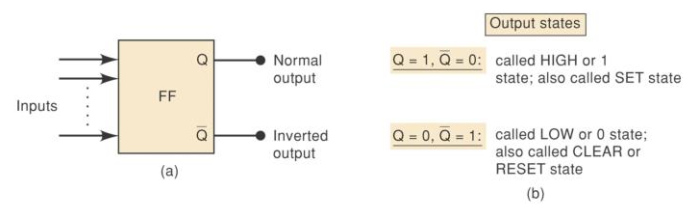
\includegraphics[scale = 0.75]{hinh6} \\
- The Flip Flop, abbreviated FF, is a key memory element.\\
- The output of the Flip Flop is Q and $\bar{Q}$. \\
- Q is understood to be the normal output, $\bar{Q}$ is always the opposite. \\
- The most basic circuit can be constructed from either two NAND gates or NOR gates.
\subsection{NAND gate latch}
- The inputs are \textbf{set} and \textbf{clear} (reset). \\
- The inputs are active low, that is, the output will change when the input is pulsed low. \\
- When the latch is set:
\begin{center}
Q = 1 and $\bar{Q}$ = 0
\end{center}
- When the latch is clear or reset:
\begin{center}
Q = 0 and $\bar{Q}$ = 1
\end{center}
\textbf{Summary of NAND latch} \\
\begin{itemize}
	\item SET = RESET = 1: Normal resting state, outputs remain in state prior to output.
	\item  SET = 0, RESET = 1: Q will go high and remain high even if the SET input goes high.
	\item SET = 1, RESET = 0: Q will go low and remain low even if the SET input goes high.
	\item SET = RESET = 0: Output is unpredictable because the latch is being set and reset at the same time.
\end{itemize}
\subsection{NOR Gate Latch}
- The NOR Gate Latch is similar to the NAND Gate Latch, except that the output Q and $\bar{Q}$ is reserved. \\
- \textbf{The inputs are active high}, that is, the outputs will change only the inputs \textbf{are pulsed high}. \\
- In order to ensure that a FF begins operation at a known level, a pulse may be applied to SET and RESET inputs when a device is powered up.
\subsection{Digital Pulses}
- In digital system, when a signal switches from a normal inactive state to the oposite (active) state, thus causing something happen in the circuit. Then the signal returns to its inactive state while the effect of the recently activated signal remains in the system. These signals are called pulses.\\
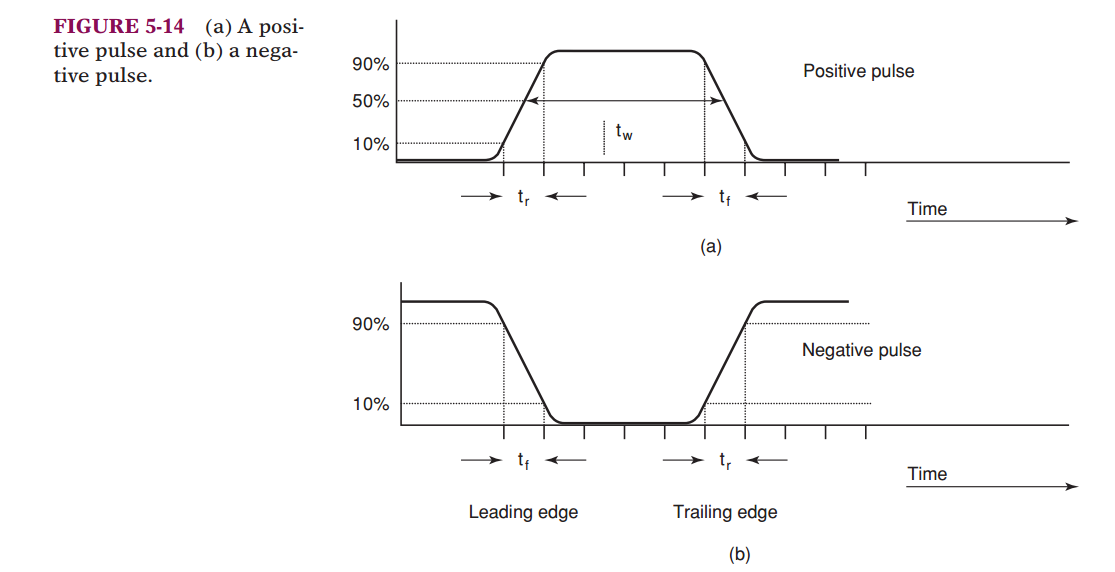
\includegraphics[scale=0.7]{hinh7}
\bigbreak
- A pulse that performs its intended function when it goes HIGH is called a positive pulse. \\
- A pulse that performs its intended funtion when it goes LOW is called a negative pulse. \\
- The transition from low to high on a positive pulse is called rise time ($t_r$). \\
- The transition from high to low on a positive pulse is called fall time ($t_f$). \\
- The transition from the beginning of the pulse is called the leading edge and the transition at the end of the pulse is called the trailing edge. \\
\subsection{Clock Signal and CLocked Flip Flop}
- Digital system can be operate either asynchronously and synchoronously:
\begin{itemize}
	\item In asynchronous system, the outputs of circuits can change state anytime one or more of the inputs change.
	\item In synchronous system, the outputs can change states at the exact time by a signal called clock. This clock signal is generally a rectangular pulse train or a square wave.
\end{itemize}
\textbf{Clock Signal}\\
- Most (if not all) of the system  outputs can change state only when the clock make a transition. \\
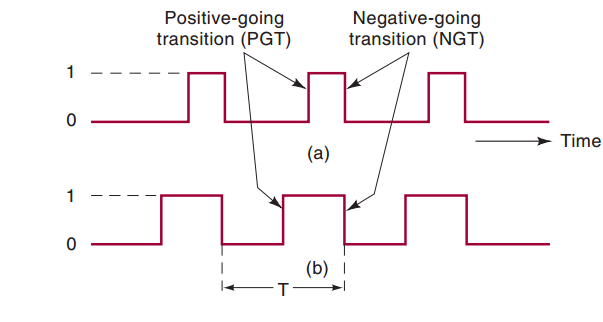
\includegraphics[scale = 0.7]{hinh8}
- A transition (also called \textit{edges}):
\begin{itemize}
	\item When the clock changes from 0 to 1, this is called the \textbf{positive-going transition (PGT)}.
	\item When the clock changes from 1 to 0, this called the \textbf{negative-going transition (NGT)}.
\end{itemize}
- Most digital system are pricipally synchronous (although there are always some asynchronous parts) because synchronous circuits are easier to design and troubleshoot.
\bigbreak
\textbf{Clocked Flip Flop} \\
\begin{itemize}
	\item CLocked FFs can change state on one or other clock transitions. Some common characteristics: \\
	- CLock inputs are labeled as CLK, CK, or CP.\\
	- A \textbf{small triangle} at the CLK input indicates that CLK input is activated with a PGT (positive-going transition). \\
	- A \textbf{bubble and a triangle} at the CLK input indicates that CLK input is activated with a NGT (negative-going transition). \\
	- Control inputs have an effect on the output only at the active clock transition (PGT and NGT). There are also called synchronous control inputs. \\
	- The control inputs get the FF outputs ready to change, but the change is not triggered until the CLK edge.
\end{itemize}
\bigbreak
\textbf{Setup Time and Hold Time} \\
- Setup time ($t_s$) is the minimum time interval before the active CLK transition that the control input must be kept at the proper level. \\
- Hold time ($t_h$) is the time after the active CLK transition during which the control input must be kept at the proper level.
\subsection{Clocked S-R Flip Flop}
- In Clocked S-R Flip Flop system, FF only change states when when a signal applied to its clock input makes a transition from 0 to 1 or from 1 to 0 (PGT and NGT). \\
- The up arrow ($\uparrow$) indicates that a PGT is required at CLK; the label $Q_{0}$ indicates the level at Q prior to the PGT. \\
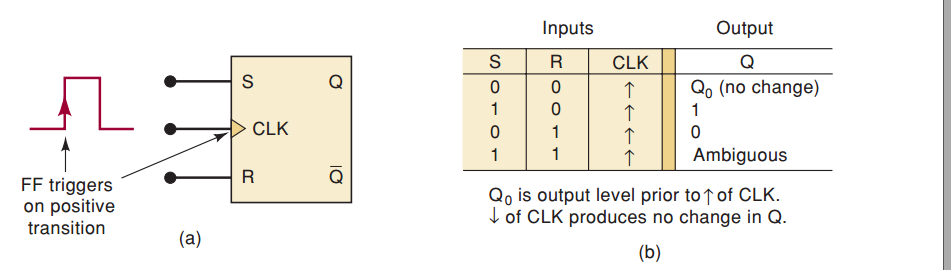
\includegraphics[scale = 0.7]{hinh10}
\bigbreak
- We can analyze these waveforms as follows: \\
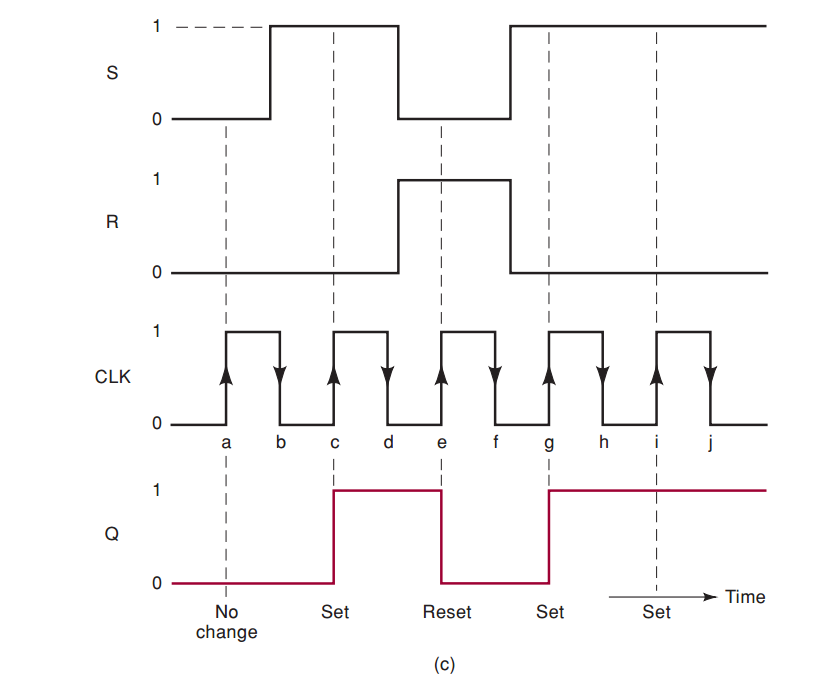
\includegraphics[scale = 0.7]{hinh9}
\bigbreak
\begin{enumerate}
	%1
	\item Initiallly all inputs are 0 and the Q output is assumed to be 0; that is $Q_0$ = 0
	%2
	\item When the PGT of the first clock pulse occurs (point a), the S and R inputs are both 0, so the FF is not effected and remains in the Q = 0 state (Q = $Q_0$)
	%3
	\item When the PGT of the second clock pulse (point c), the S = 1 and R = 0. Thus the FF set to 1 state at the rising edge of this clock pulse.
	%4
	\item When the third clock pulse makes its positive transition (point e) S = 0 and R = 1. Thus it causes the FF set to 0 state.
	%5
	\item At the fourh pulse set the FF once again to the Q = 1 state (point g) because S = 1 and R = 0 when PGT occurs
	%6
	\item The fifth pulse also find that S = 1 and R = 0 at PGT occurs so the FF remains state.
	%7
	\item The case that S = R = 1 should not be used because it results in an ambiguous condition.
	%8
	\item It should be noted that those waveforms that the FF is \textbf{not effected} by the NGT of the clock pulses. Also note that the S and R levels have no effects on the FF, except upon the occurence of the PGT \textbf{in PGT transitions}
	%9
	\item For the NGT transition the FF operate at the same manner at PGT transition, except the output can change states only on the falling edge of the clock pulse
\end{enumerate}
- As a general rule for stable flip flop triggering, the clock pulse rise and fall time must be very short, around typically 2 - 5 ns. \\
\subsection{Clocked J-K Flip Flop}
- The J and K inputs control the state of the FF in the same way as the S and R inputs do for the clocked S-R flip flop, except 1 difference that when J = K = 1 condition \textbf{does not result} in ambiguous output. In this condition, the FF will always go to its opposite side of the clock signal, this is called \textbf{toggle mode} of the operation.\\
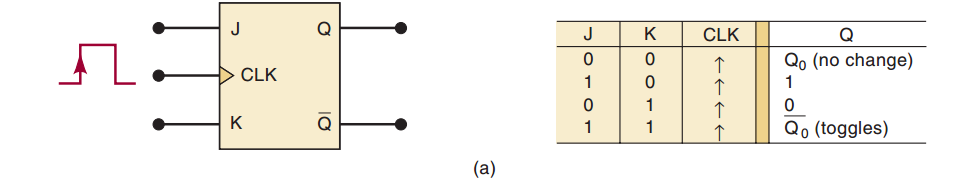
\includegraphics[scale = 0.6]{hinh11}
\bigbreak
- The operation of the J-K Clocked Flip Flop is the same as the S-R Clocked Flip Flop , except when J = K = 1 at the PGT transition the output will change to the opposite state. \\
- Also in NGT, the operation is still same as PGT when clock is triggered in NGT.\\
- In edge-triggered J-K Flip Flop, CLK* must be high for FF to change states. This condition only occurs at the edge of a CLK transition
\subsection{Clocked D Flip FLop}
- Unlike the S-R and J-K Clocked FLip Flop, this flip flop has only one synchronous control input, \textit{D}, which stands for data. \\
- The operation of the D  CLocked Flip Flop is very simple: Q will go as the same state on the D input when a PGT occurs at CLK. \\
- A negative-edge-triggered D flip flop operates in the same way and Q will take on the value of D when a NGT occurs at CLK. \\
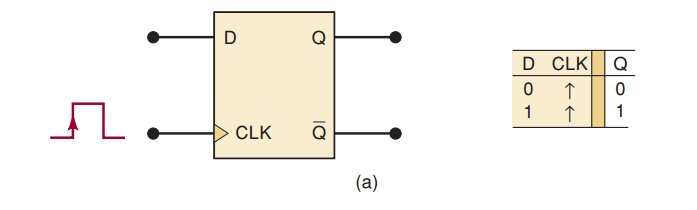
\includegraphics[scale=0.6]{hinh12}
\subsection{D Latch (Transparent Latch)}
-  The edge trigggered D Flip Flop uses an edge-detector circuit to ensure that the output will repond to the D input only when the active transition of the clock occurs. The latch that its edge-detector is not used called the D latch.
\begin{itemize}
	\item One data input.
	\item The clock has been replaced by an ENABLE (EN).
	\item The device is not edge-triggered.
	\item When EN = 1; the output follows the change of input.
	\item When EN = 0; wheither D changes or not Q will stay at their current level (no change).
\end{itemize}
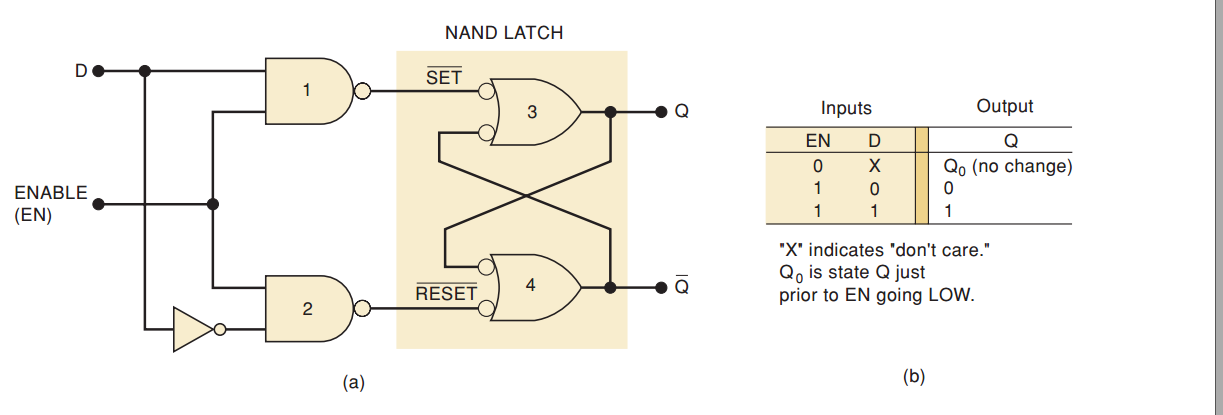
\includegraphics[scale = 0.6]{hinh13}
\bigbreak
- Logic symbol of D latch: \\
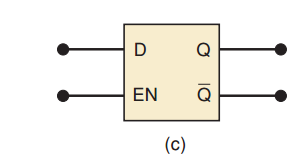
\includegraphics[scale = 0.65]{hinh14}
\subsection{Asynchronous Inputs}
\begin{itemize}
	\item For the clocked flip flop, the S-R, J-K and D inputs have been reffered as \textbf{synchronous inputs}
	\item Most clocked FF also have one or more asynchronous inputs that operate independently of the synchronous inputs.
	\item These asynchronous inputs can be used to set FF to the 1 state of clear (reset) and FF to 0 state at \textbf{any time, regardless conditions of inputs}.
	\item State in another way, the asynchronous inputs are \textbf{overide inputs}
\end{itemize}
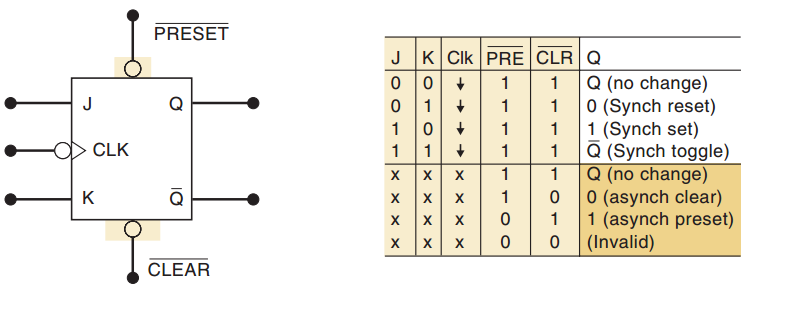
\includegraphics[scale = 0.65]{hinh15.png}
\bigbreak
- $\overline{PRESET} = \overline{CLEAR} = 1$: The asynchronous inputs are inactive and the output depend only on CLK transitions. \\
- $\overline{PRESET} = 0; \overline{CLEAR} = 1$: The $\overline{PRESET}$ is activated and Q = 1 (no matter what conditions). The CLK inputs cannot affect the FF while $\overline{PRESET}$ = 0. \\
- $\overline{PRESET} = 1; \overline{CLEAR} = 0$: The $\overline{CLEAR}$ is activated and Q = 0 (no matter what conditions). The CLK inputs cannot affect the FF while $\overline{CLEAR}$ = 0. \\
- $\overline{PRESET} = \overline{CLEAR} = 0$: Ambiguous response. \\
\section{Flip Flop Timing Consideration}
\subsection{Setup and Hold Times}
- Setup time and Hold time represent for reliable FF triggering. In IC's datasheet will always spectify the minimum values of $t_s$ and $t_h$
\subsection{Propagation Delays}
- Whenever a signal is to change the state of a FF's output, there is delay from the time the signal is applied to the time when the output makes its change. \\
- The delay is measured between 50 percent points on the input and output waveform.
- Modern IC flip-flops have propagation delay that ranges from a few ns to 100 ns.
\subsection{Maximum Clocking Frequency ($f_{Max}$)}
- This is the highest frequency that may be applied to the CLK input of a FF and still have it triggerreliably.
\subsection{CLock Pusle HIGH and LOW time}
- Clock Pulse HIGH is the time when the CLK is kept at HIGH before goes LOW. \\
- CLock Pulse LOW is the time when the CLK is kept at LOW before goes HIGH. \\
\subsection{Asynchronous active pulse width}
- The minimum time that PRESET or CLEAR must be held for the FF to set of clear reliably.
\subsection{Clock Transition Time}
- For reliable triggering, the clock waveform transition times (rise and fall time) should be kept be very short. If the clock signal takes too long to make the transition from 1 level to another, the FF will trigger eratically.
- The transition time should be $\le$ 50 ns for TTL devices and $\le$ 200 ns for CMOS
\section{Potential Timing Problem in FF circuit}
- When the output of one FF is connected to the input of another FF and both devices are triggered by the same clock, there is a potential timing problem. \\
- Propagation time delay may cause unpredictable outputs.
- The problem can be reduced due to low hold time.
\section{Flip Flop Synchronization}
- Most system are primarily synchronous in their operation most of the signals will change states in synchronism with the clock transition. \\
- The randomness by asynchronous can produce unpredictable result.
\section{Data Storage and Transfer}
- Most common of the flip flop is for storage and information. \\
- The data is stored in groups is called \textbf{register}. \\
- The operation most often performed in data that is stored in a FF or a register is the \textbf{data transfer} operation, the operation involves the transfer from one FF or register to another. \\
\begin{figure}
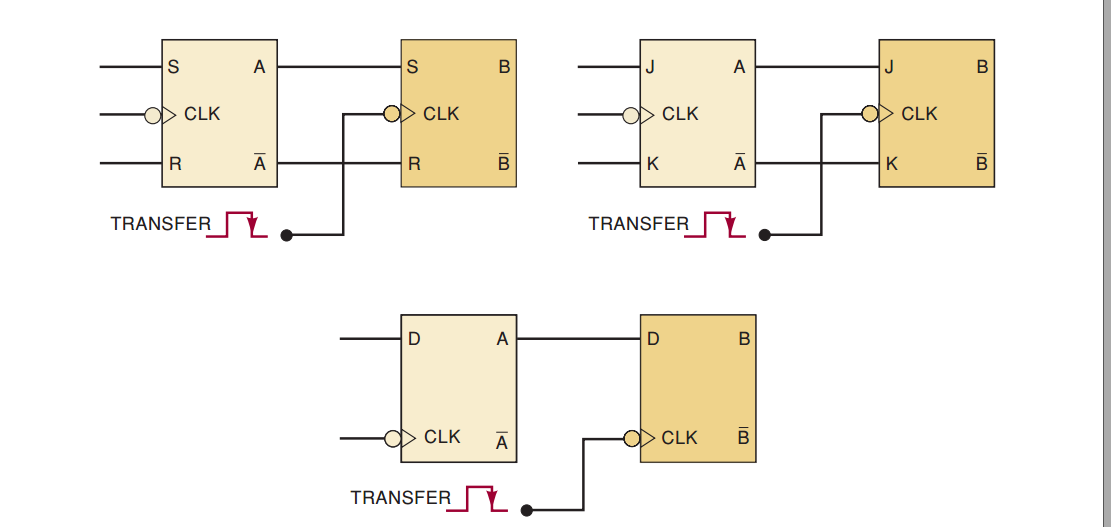
\includegraphics[scale = 0.6]{hinh19}
\label{Synchronous Data Transfer of S-R, J-K, D flip flops}. \\
\end{figure}
\\
- For Asynchronous Data Transfer, in the figure, the inputs respond to LOW level. When the \textbf{Transfer enable} is LOW, the two NAND outputs is HIGH. \\
- When the \textbf{Transfer enable} is HIGH, one of two NAND outputs is LOW, depends on the states of A and $\overline{A}$. This LOW value (SET or RESET) will make FF B as same state with FF A. \\
- Asynchronous is also called as \textbf{jammed transfer}. \\
\subsection{Paralled Date Transder}
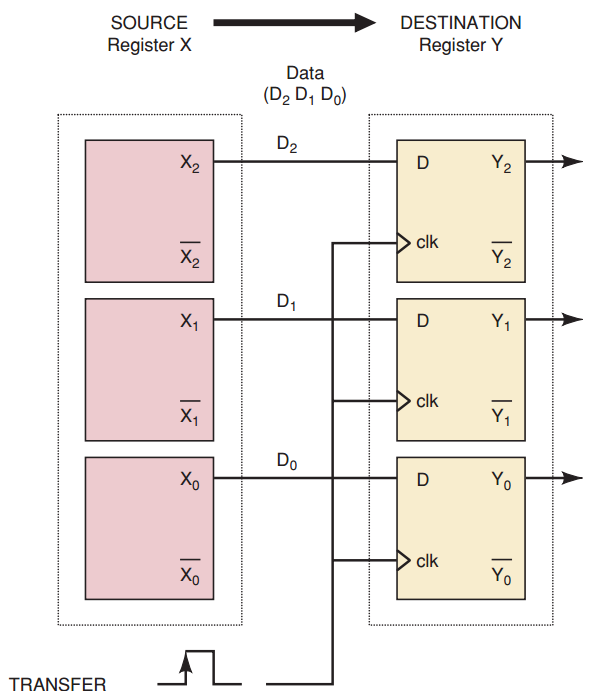
\includegraphics[scale = 0.6]{hinh20} \\
\begin{itemize}
	\item The transfer from X register into Y register is a synchronous transfer. \\
	\item The transfer is called \textbf{parallel transfer} due to the contents of $X_2 , X_1$ and $X_0$ and is transfer simultaneously into $Y_2, Y_1$ and $Y_0$.
	\item If a \textbf{serial data} transfer were performed, the content of X register would be transfered to Y register one bit at a time.
\end{itemize}
\section{Serial data Transfer: Shift Registers}
\bigbreak

\section{Arithmetic Operation}
\subsection{Binary Addition}
\begin{itemize}
	\item 0 + 0  = 0
	\item 0 + 1 = 1
	\item 1 + 1 = 0 + carry 1
	\item 1 + 1 + 1 = 1 + carry 1
\end{itemize}
- The carry 1 will be added to the next position, which is add to the left. \\
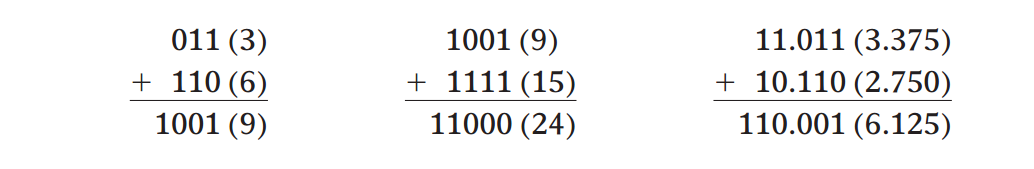
\includegraphics[scale = 0.6]{hinh21}
\bigbreak
- The carry 1 from the operation will be added to next position. \\
\subsection{Represent Signed number}
- By adding 2 numbers 0 and 1, we can represent the \textbf{sign} of the number which is called \textbf{sign bits}
\begin{itemize}
	\item To represent the positive number, we add \textbf{0} before the MSB of the binary number.
	\item To represent the negative number, we add \textbf{1} before the MSB of the binary number.
\end{itemize}
- But that is the way to show the sign of the binary number. In computer do not normally use it because the circuit implementation is complex than other systems. \\
Ex: $52_{10} = 0110100_{2}$, we cannot assume that $ - 52_{10} = 1110100_{2}$. The result is different. \\
- In this case, \textbf{2's complement system} is used to represent the signed number.
\begin{enumerate}
	%1
	\item 1's complement: \\
	- First, we start with the 1's complement form: \\
	\begin{itemize}
		\item The 1's complement of the binary number is obtained by changing each 0 to 1 and each 1 to 0.
		\item 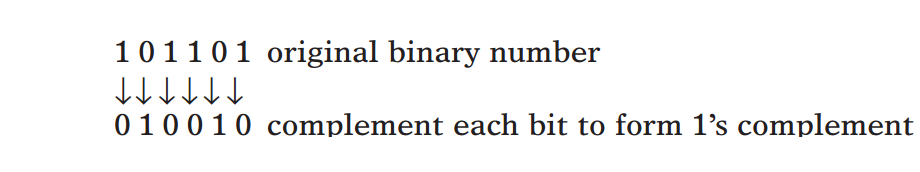
\includegraphics[scale = 0.6]{hinh22}
	\end{itemize}
	%2
	\item 2's Complement Form: \\
	- The 2's complement form is formed by taking 1's complement and then adding 1 to the LSB of the binary number. \\
	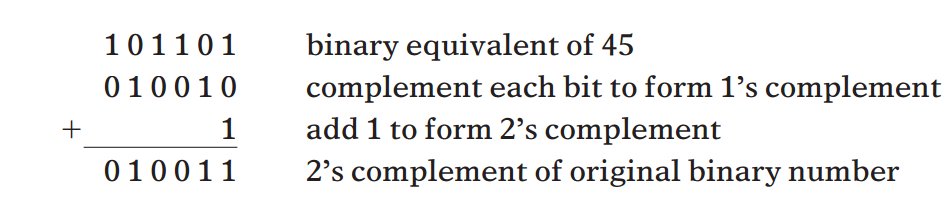
\includegraphics[scale = 0.6]{hinh23}
	\bigbreak
	%3
	\item Represent the signed number by 2's Complement form: \\
	- This method can also use in unsigned number.
	\begin{itemize}
		\item Take 1's complement of the binary number.
		\item Add to LSB.
	\end{itemize}
\subsection{Sign Extension}
- When extend the binary number to another more bits, we duplicate the sign bit. \\
	Ex: We have 4 bits of $12_{10}$ is $1100$, add \textbf{sign bit} 0 to MSB then we append 0 until we get the possible bits we want to extend.
\end{enumerate}
\subsection{Negation}
- \textbf{Negation} is the operation of converting a positive number to its negative equivalent or a negative to its positive equivalent.
\subsection{Special Cases in 2's Complement Representation}
- Signed Number contains 1 as sign bits and 0 as its magnitudes.\\
- The complete range of signed number have N magnitude bits is:
\begin{center}
	$-2^N$ to $+ (2^N -1)$
\end{center}
$\rightarrow$ There are a total $2^{N+1}$ different values, including zero.\\
Ex: Some Example: \\
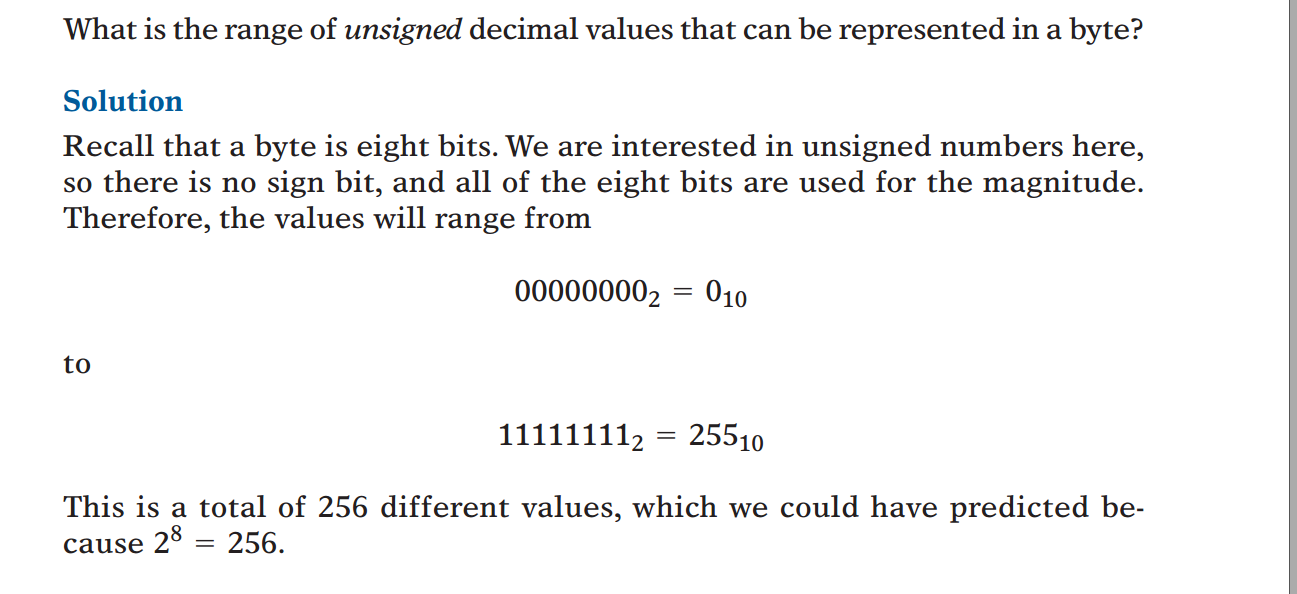
\includegraphics[scale = 0.6]{hinh24}
\bigbreak
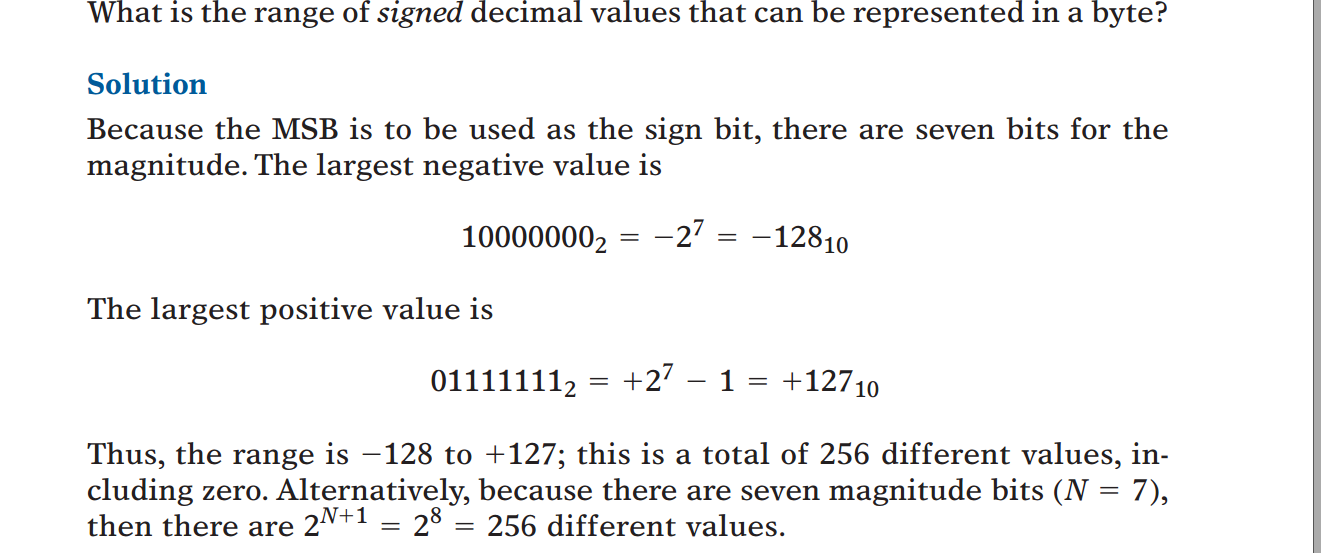
\includegraphics[scale = 0.6]{hinh28}
\bigbreak
\subsection{Addition in the 2's Complemetn System}
\begin{enumerate}
	%1
	\item Two Positve Number: \\
	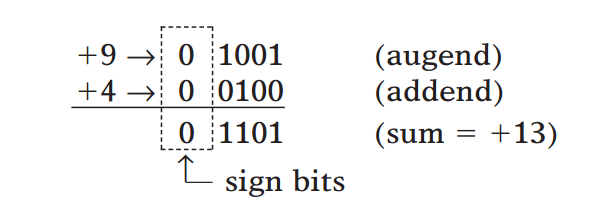
\includegraphics[scale = 0.6]{hinh25}
	%2
	\item Positve and Negative smaller number: \\
	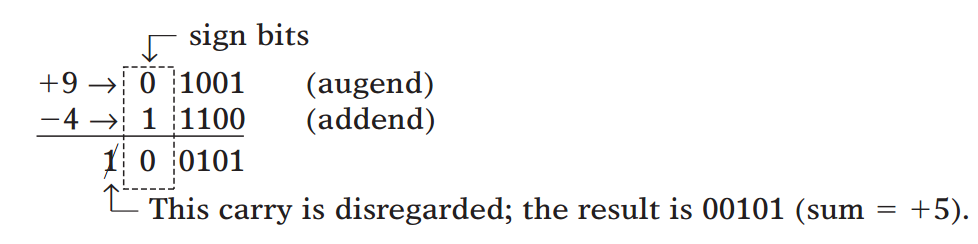
\includegraphics[scale = 0.6]{hinh26}
	%3
	\item Positive and Negative larger number: \\
	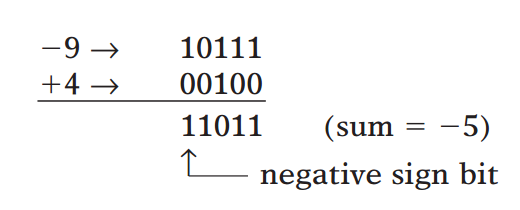
\includegraphics[scale = 0.6]{hinh29}
	%4
	\item Two Negative Number: \\
	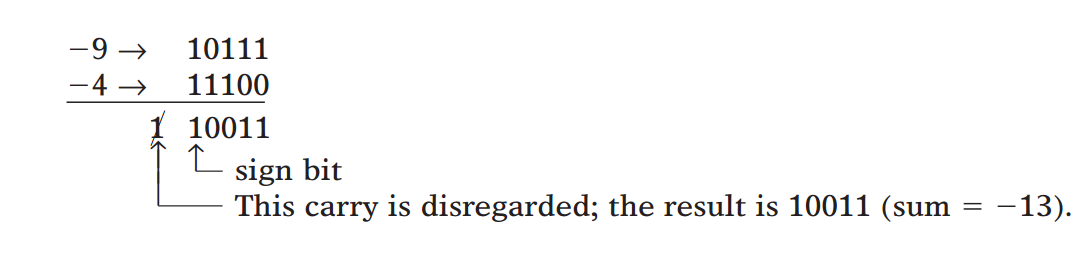
\includegraphics[scale = 0.6]{hinh27}
\end{enumerate}
\subsection{Subtraction in 2's Complement System}
- When subtracting one binary number (the subtrahend) from another binary number (the minuend) :
\begin{itemize}
	\item Negate the subtrahend: This will change the subtrahend to its equivalent value of opposite sign.
	\item Add the result to minuhend
\end{itemize}
\subsection{Arithmetic Overflow}
- Arithmetic Overflow occurs when we add 2 positive or negative binary number which the result require more than bits and therefore \textbf{overflow} into the sign-bit position
- When we perform the subtraction, the \textbf{overflow} occurs when the subtrahend is negated and become the addition berween 2 positive numbers.
\subsection{Multiplication of Binary Number}
\begin{enumerate}
	%1
	\item Multiplication between 2 binary number:
	- To perform the multiplication between 2 binary number we perform the multiplication between multiplicand and the LSB of multiplier, the result is written down as the first partial product. \\
	- Then we come with the second number from thw left of the equation, the second result is written down as second partial product, the second result should be \textbf{shifted} 1 bit to the left. \\
	- Then we try with the third and fourth ... after that, perform the addtion with partial products to get the final result. \\
	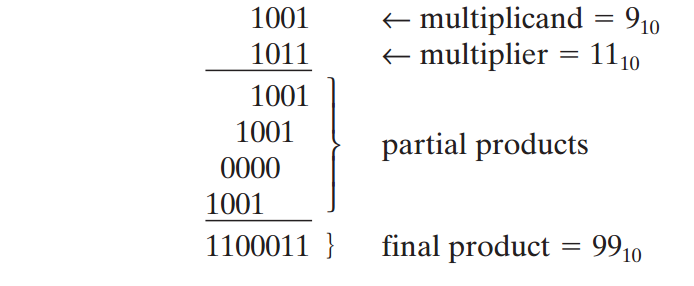
\includegraphics[scale = 0.6]{hinh30}
	\bigbreak
	%2
	\item Multiplication between 2's Complement Form: \\
	- When 2 numbers is negative in multiplication, we negate both 2 number then perform the equation. \\
	- When one number is positive and the other is negatve, we negate the negative one then perform the equation and the final result should be negated.
\end{enumerate}
\subsection{Binary Devision}
 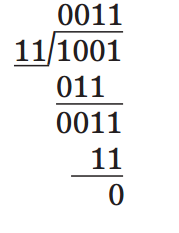
\includegraphics[scale = 0.6]{hinh31} \\
 - The figure below shows the division between $1001_{2}$ and $11_{2}$ and the quotient of the division is $0011_{2}$. \\
 - To perform the binary devision, follow the step: \\
 \begin{itemize}
 	\item As we have the devisor is 11, first take the first number in the left to divide for 11. Consider 1001, we take 1 / 11, because 1 is < 11 then the result is 0, write 0 as the result. Then continue with 10, 100 and 1001, if the dividend is larger than the devisor the result will come to 1.
 	\item If the result is 1, perform the multiplication between 11 to 1 is 11, write 11 below 100 (dividend) and the perform the binary substraction to get the remainder, after that get the last 1 from the dividend to the remainder, repeate the step
\end{itemize}
\subsection{BCD Addition}
\begin{enumerate}
	%1
	\item Sum equals 9 or less: \\
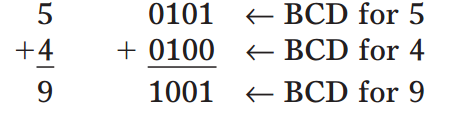
\includegraphics[scale = 0.6]{hinh32}
\bigbreak
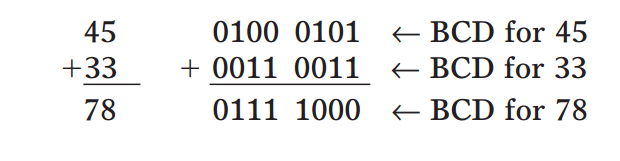
\includegraphics[scale = 0.6]{hinh33.png}
	%2
	\item Sum greater than 9: \\
	- When peform the addition between BCDs that produce the sum that is greater than 9, we should add 6 bits to the sum ($6_{10} = 0110_{2}$) to get the result in 4 bits. \\
	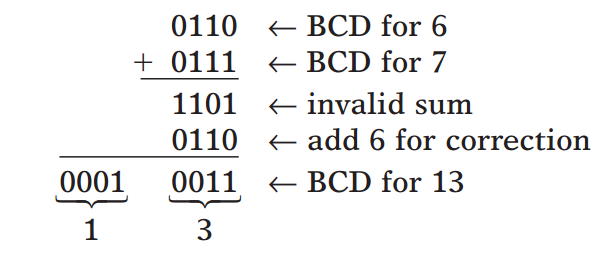
\includegraphics[scale = 0.6]{hinh34}
	\bigbreak
	- Another example: \\
	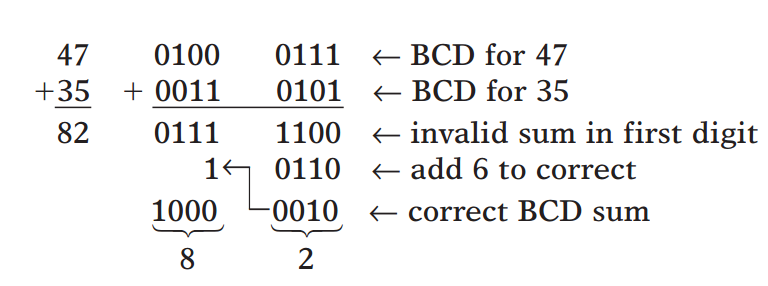
\includegraphics[scale = 0.6]{hinh35}
\end{enumerate}
\section{Hexedecimal Arthimetic}
\subsection{Hex Addition}
- To perform the Hexadecimal Addition, follow the procedure: \\
\begin{itemize}
	\item Add the 2 hex digit in decimal, mentally inserting the decimal equivalent for those digits larger than 9.
	\item If the sum is 15 or less, it can be directly expressed in hex digits( A, B, C, D, F).
	\item If the sum is larger than or equals 16, substract 16 and get carry 1 to the next position.
\end{itemize}
\subsection{Hex Substraction}
- The procedure to perform the hex substraction is similar to the binary substraction. \\
- To change the hex digit to its 2's complement form, we take FFF substracts to the hex number then add 1. \\
- After that take the addtion with the hex number in 2's complement form to get the result. \\
\section{Arithmetic/Logic Unit (ALU)}
- All arithmetic operation take place in the \textbf{Arthimetic/ Logic Unit} (ALU) of a computer. \\
- The arithmetic/logic unit contains at least 2 flip-flop register: the B register and the \textbf{accumulator register} \\
- The operation follow: \\
\begin{itemize}
	\item The control units receives an instruction (from the memory unit) specify that a number stored in a particular memory location (address) is to be added to the number represently stored in the \textbf{accumulator register}.
	\item The number to be added is transfer from memory to the B register.
	\item The number in B register and the number in the \textbf{accumulator register} are added together in the logic circuit. The result is sent to the accumulator to be stored.
	\item The new number in the accumulator can remain there so that another number can be added to it or if the particular arithmetic process is finished, it can be transfer to memory for storage.
\end{itemize}
\bigbreak
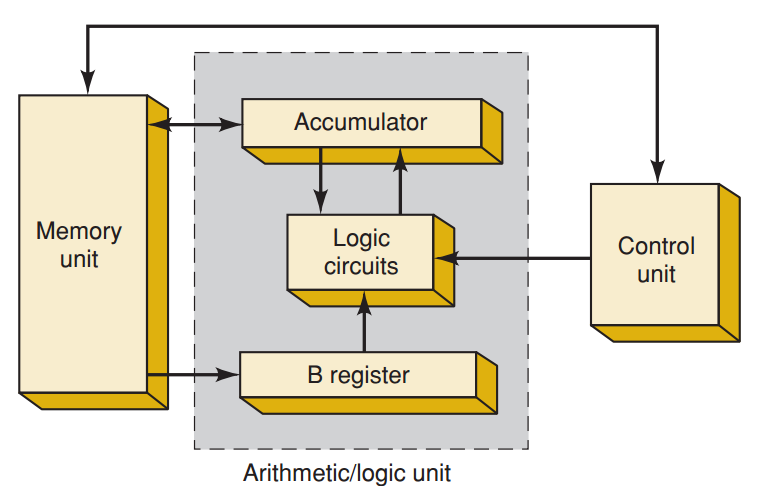
\includegraphics[scale = 0.6]{hinh36}
\subsection{Parallel Binary Adder}
- To perform the addition between two binary digits we perform the addition of each digit, the carry after the addition will be added to the next position. \\
- So that we can calculate the sum \textbf{parallel} with add carry to the next position. This is called \textbf{Parallel Binary Adder}. \\
- The whole process is performed in logic circuit called \textbf{full adder}. \\
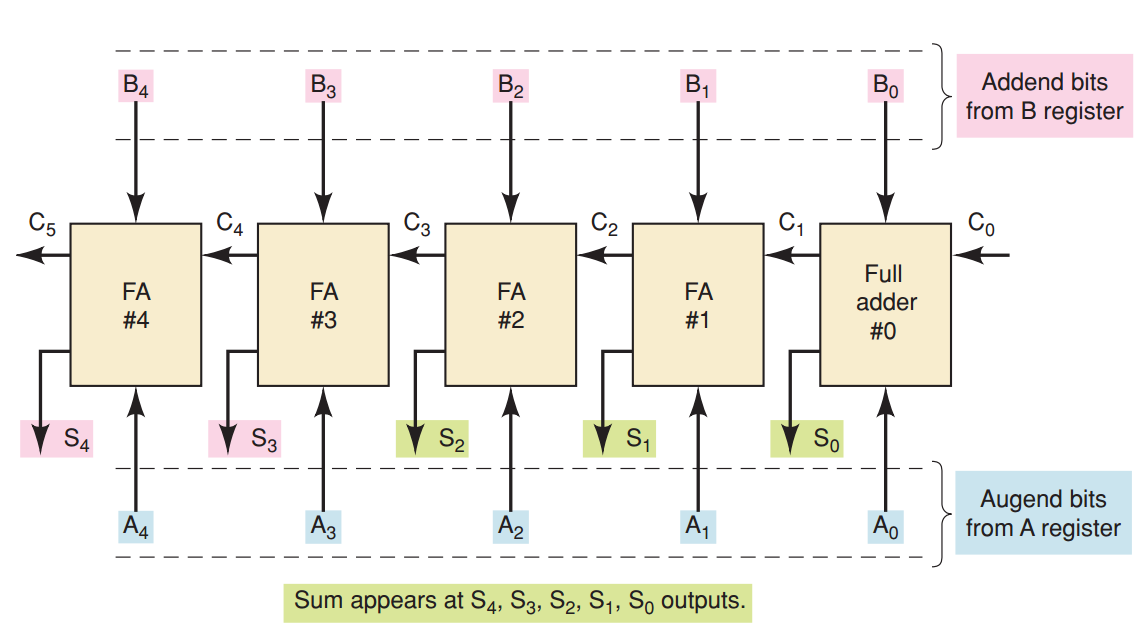
\includegraphics[scale = 0.6]{hinh37}

\section{Counter and Register}
\subsection{Asynchronous Counter}
- In asynchronous Counter:
\begin{itemize}
	\item The clock pulses are applied to the CLK input of flip-flop A.
	\item The output of the flip-flop A acts as the CLK input for flip-flop B, same with C and D.
	\item FF outputs D, C, B and A represents a 4 bits binary number, with D as MSB
\end{itemize}
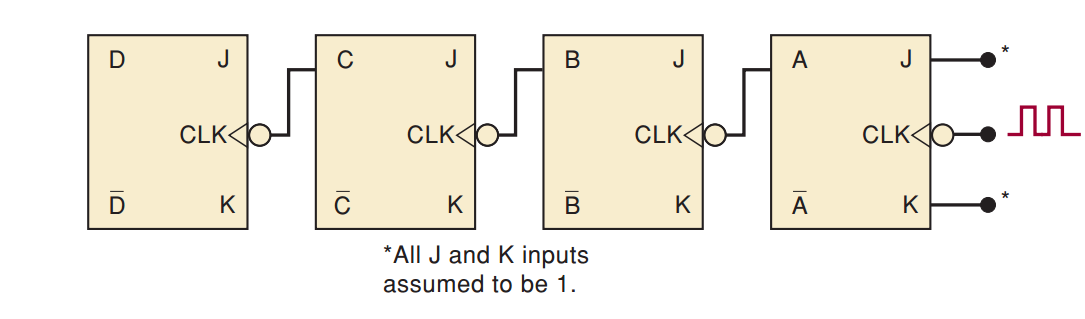
\includegraphics[scale = 0.6]{hinh38}
\bigbreak
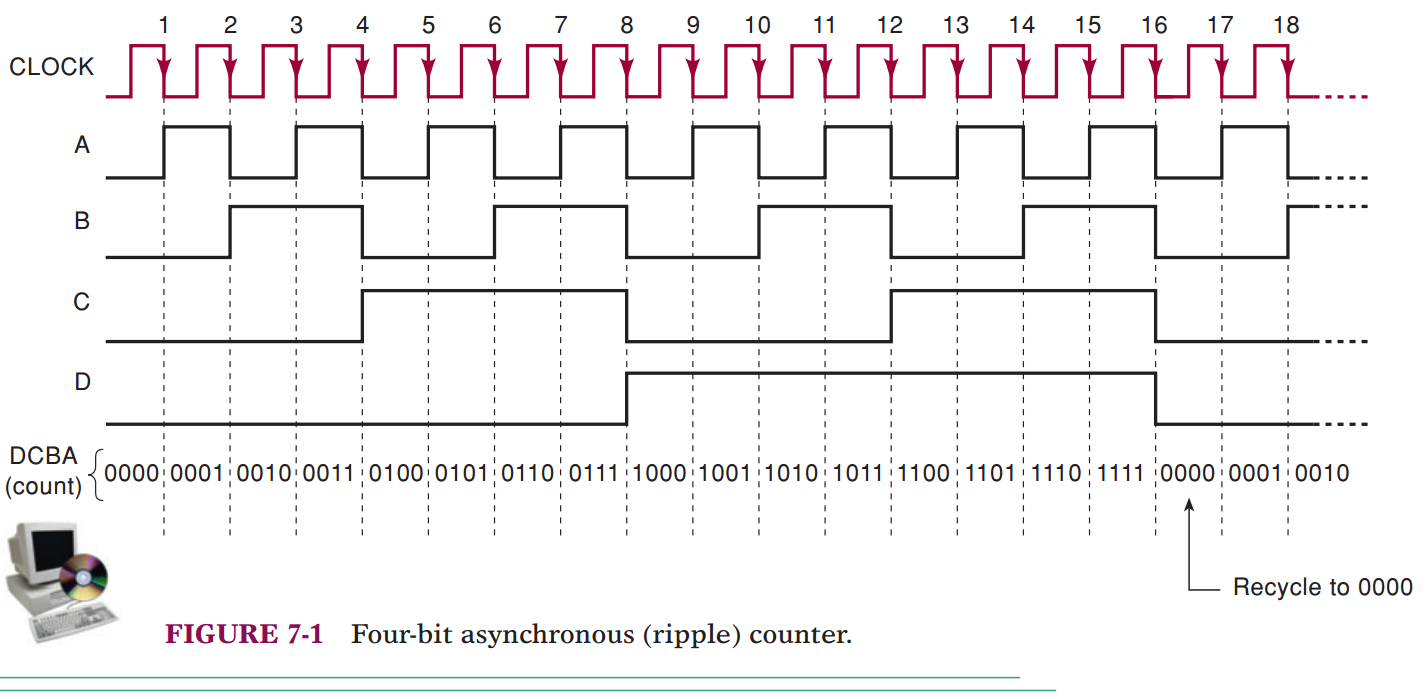
\includegraphics[scale = 0.6]{hinh39}
\bigbreak
\subsection{Signal Flow}
- In the counter circuit, CLK inputs of each flip flop are on the right, the ouputs are on the left, and the input clock input signal is shown comming to the right. \\
\subsection{MOD Number}
- \textbf{MOD} number is generally equal to the number of states that the counter goes though in each complete cycle before it rises back to its starting state. \\
\begin{center}
MOD number = $2^{n}$
\end{center}
\textit{When n is the number of each FFs connected}
\subsection{Frequency Division}
- In the basic counter, each FF provides an output waveform that is exactly the \textbf{half} frequency of the waveform at its CLK input. \\
- In any counter, the signal at the output of the last FF (MSB) will have the frequency equal to the input clock frequency divided by the \textbf{MOD} number of the counter. \\
\subsection{Propagation Delay in the Ripple Counter}
- Ripple counter is the simplest type of the binary counter because they require the fewest components to produce a given counting operation. \\
- Since each FF triggered by the transition at the output will have propagation delay time of each FF. That means the second FF will not respond until the first FF receives an active clock transition; the third FF will not respond until the 2 $\times$ propagation delay after that clock transition. \\
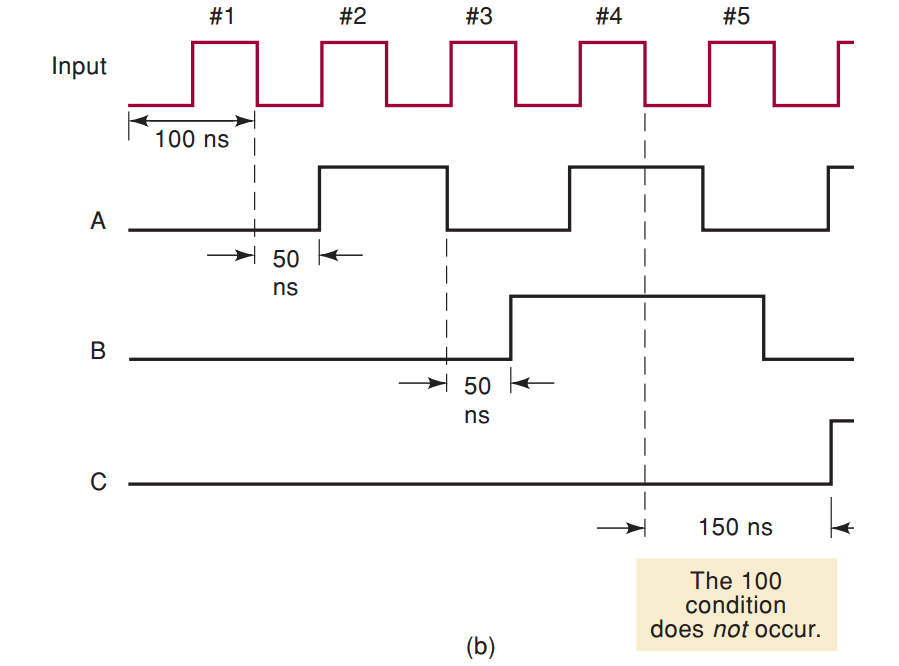
\includegraphics[scale = 0.6]{hinh40}
\bigbreak
- For proper counter we need :
\begin{mybox}
	\begin{center}
		$T_{clock} \ge N \times t_{pd}$
	\end{center}
\end{mybox}
\textit{Where N = number of FFs} \\
\bigbreak
- For the frequency of clock input:
\begin{mybox}
	\begin{center}
		$f_max = \dfrac{1}{N \times t_{pd}}$
	\end{center}
\end{mybox}
\subsection{Synchronous (PARALLEL) Counter}
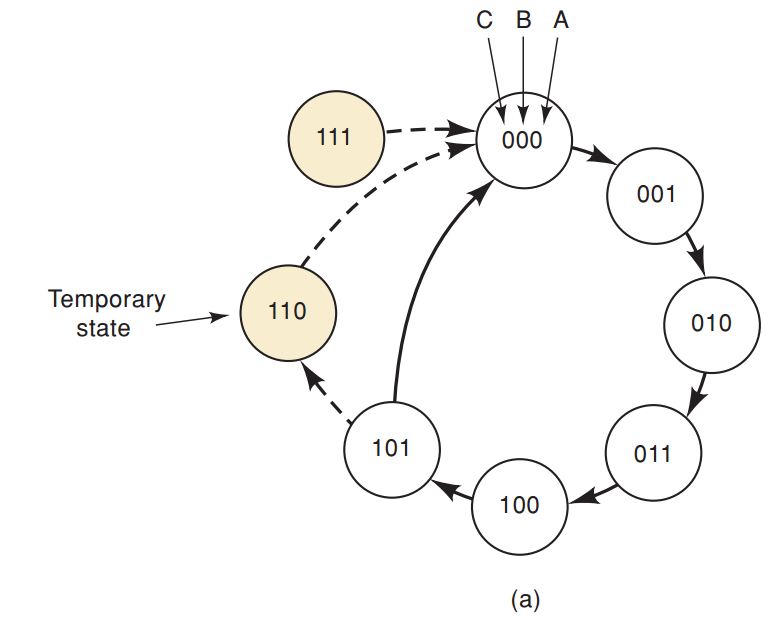
\includegraphics[scale = 0.6]{hinh41}
\bigbreak
- Since the problem of propagation delay caused ripple counter that all FFs cannot cange simultaneously. \\
- Synchronous (Parallel Counter): The input pulses are applied to all the FFs. \\
- Some difference between Synchronous and Asynchronous Counter: \\
\begin{itemize}
	\item The CLK inputs of all the FFs are connected together so that the input clock signal is applied to each FF simultaneously.
	\item Only the flip flop A (LSB) has its J, K inputs pernamently at the HIGH level.
	The J, K of the other FFs are driven by some combination of FF outputs.
	\item The synchronous counter requires more circuitry than does the asynchronous counter.
\end{itemize}
\textbf{Circuit Operation}
- The A fip flop changes states at each NGT, its J and K are pernamently HIGH so that it will toggle at on each NGT of the clock input. \\
- The B flip flop changes states at A = 1 and C flip flop changes states at A = B = 1, so on with the flip flop D. \\
\begin{center}
\textit{\textbf{Each FF should have its J and K inputs connected so that they are HIGH only when the outputs of all lower-order FFs are in the HIGH state.}}
\end{center}
- The total delay of Synchronous Counter equals the time of one FF toggle + the time of the logic AND gate to reach the J, K inputs.
\begin{mybox}
	\begin{center}
		total delay = FF $t_{pd}$ + AND gate $t_{pd}$
	\end{center}
\end{mybox}
\subsection{Counter with MOD number $\le 2^{n}$}
- The basic counter can be modified to produce MOD numbers less than $2^{n}$ by allowing the counter to \textbf{skip states} that are normally part of the counter sequence. \\
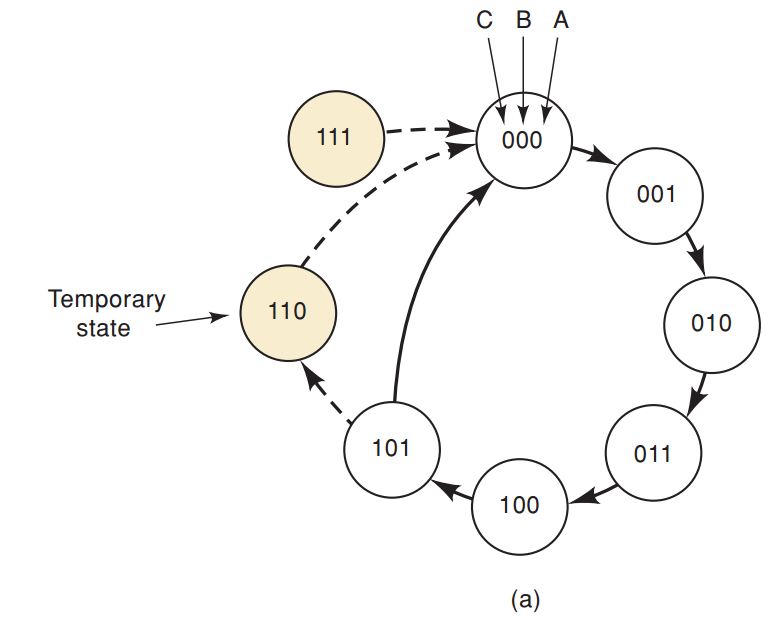
\includegraphics[scale = 0.6]{hinh41}
\bigbreak
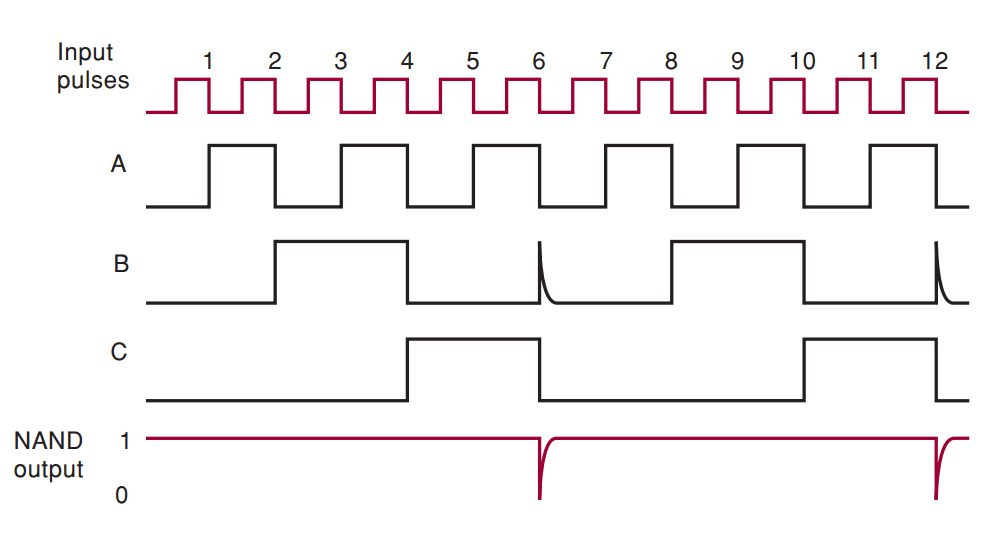
\includegraphics[scale = 0.6]{hinh42}
\bigbreak
\begin{itemize}
	\item The NAND output us connected to the asynchronous CLEAR inputs of each FF. When the NAND output is HIGH, it is no effect to the counter, but when it goes LOW it will active the CLEAR and the counter immediately goes to 0 state.
	\item The inputs of NAND gates are the outputs of B and C flip flops and so the NAND output will go LOW whenever the B and C equal 1.
	\item The counting sequence: \\
		\begin{center}
			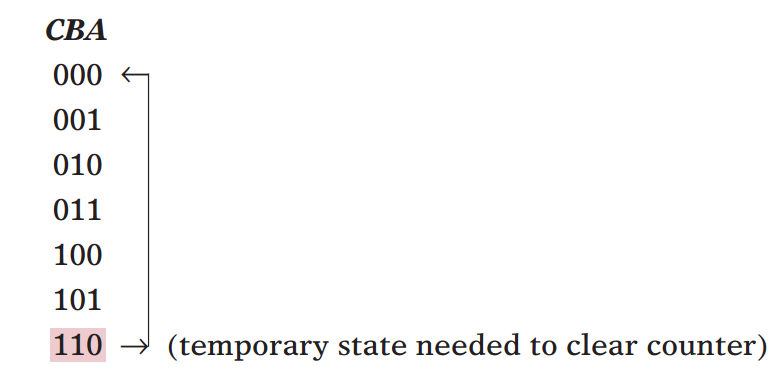
\includegraphics[scale = 0.6]{hinh43}
		\end{center}
\end{itemize}
\subsection{State Transition Diagram}
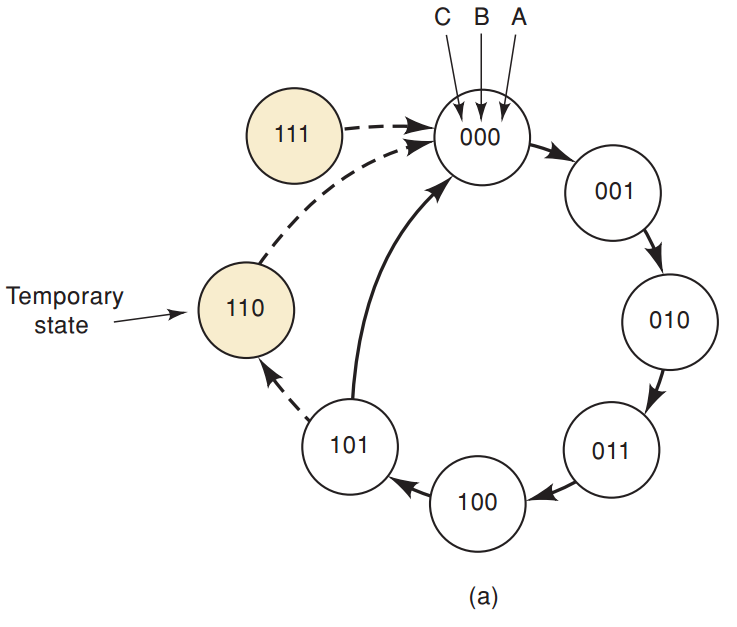
\includegraphics[scale = 0.6]{hinh44}
\bigbreak
\subsection{Displaying Counter States}
- We use individual indicator LEDs to have a visible display on how the counter changes for each FF output. Each FF output is connected to an INVERTER whose output provides the current path for LED. \\
- When the output A is HIGH, the INVERTER outputs goes LOW and the LED turns ON, the LED turning on indicates the A = 1. \\
- When output A is lOW, the INVERTER output is HIGH and the LED turns OFF, the led turning off indicates A = 0. \\
\subsection{Decade Counter / BCD Counter}
- A decade counter is any counter that has 10 distinct states, no matter what the sequence. \\
- BCD counter is the decade counter uses only 10 BCD code groups 0000, 0001, ...., 1001. \\
\begin{center}
\textit{\textbf{Any MOD 10 counter is decade counters and any decade counters that count from 0000 to 1001 are BCD counter}}
\end{center}
\bigbreak
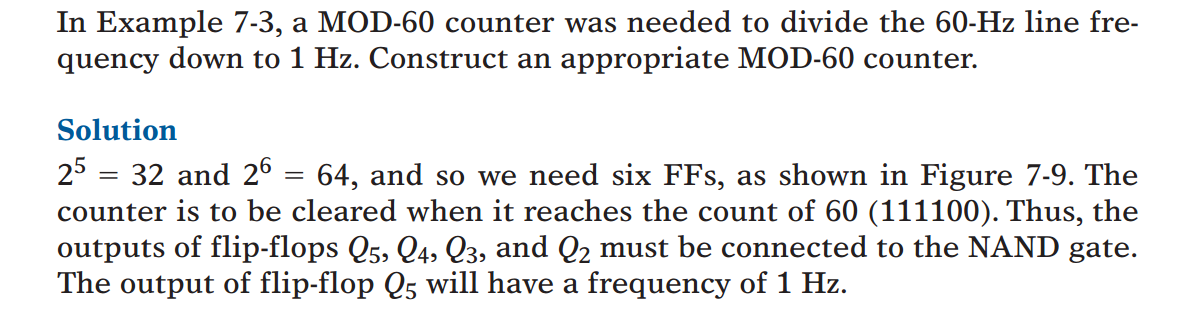
\includegraphics[scale = 0.6]{hinh45}
\bigbreak
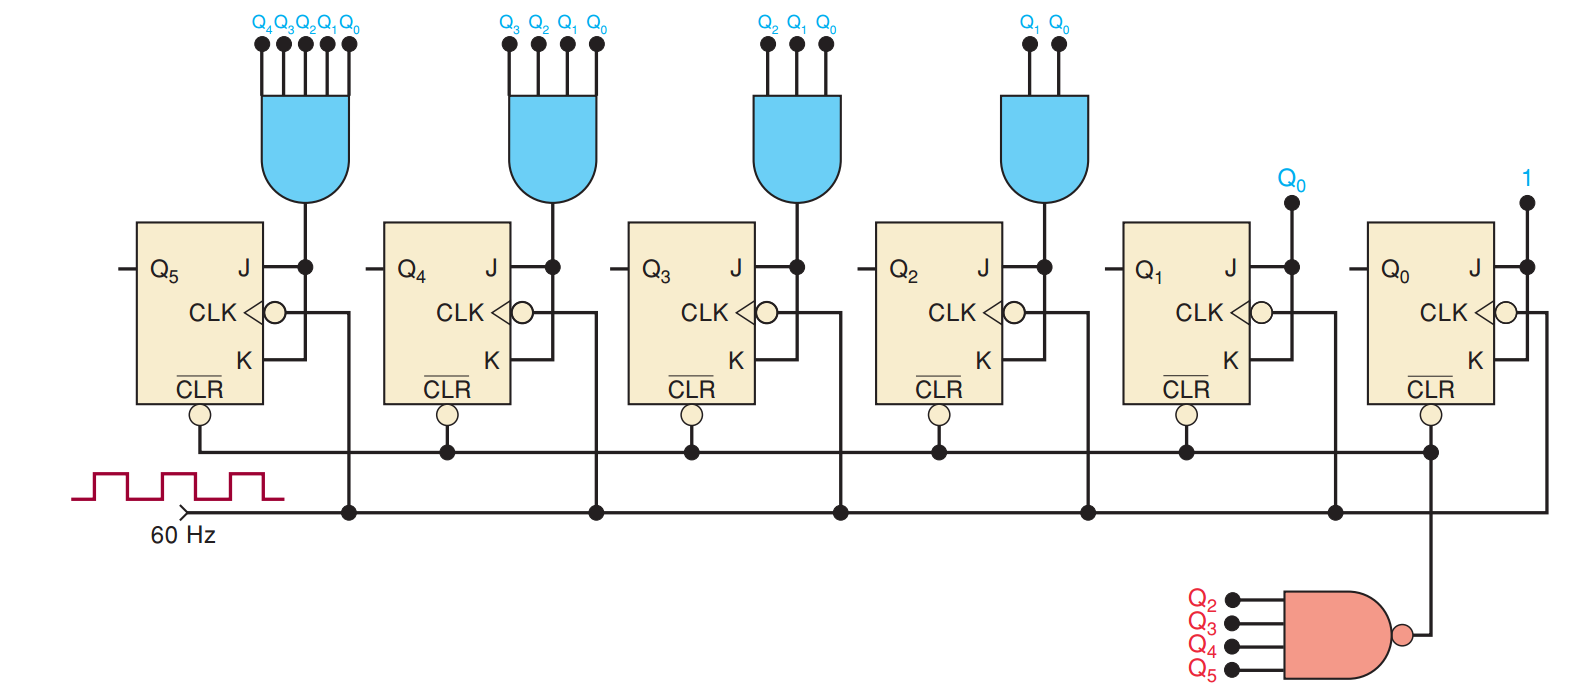
\includegraphics[scale = 0.6]{hinh46}
\bigbreak
\subsection{Synchornous Down and Up/Down Counter}
- A synchronous up counter has the output of the FFs comes from the positive value. \\
- A synchronous down counter has the output of the FFs comes from the negative value. \\
\textbf{Up/Down Counter} \\
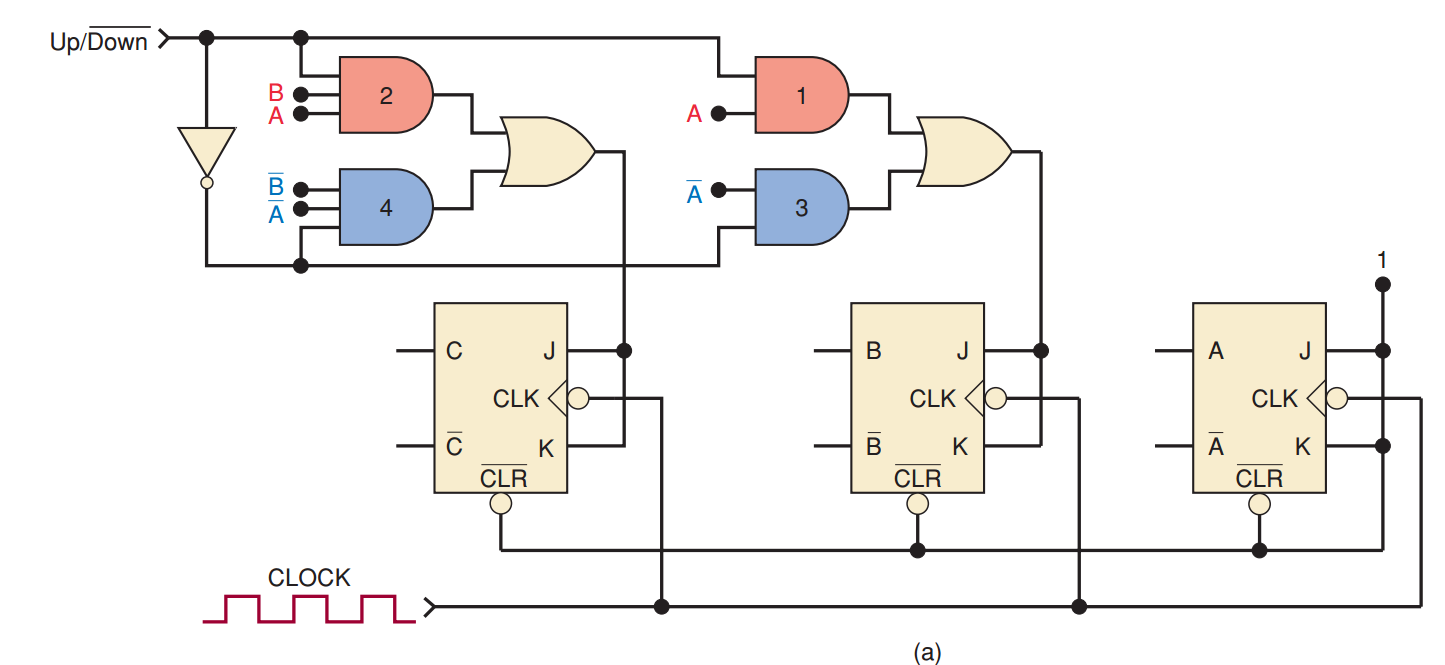
\includegraphics[scale = 0.6]{hinh47}
\begin{itemize}
	\item When Up/Down is held HIGH, AND gates 1 and 2 are enabled while AND gates 3 and 4 ar disabled. This allows the A and B outputs through gates 1 and 2 to the J, K inputs of FFs of B and C.
	\item When Up/Down is held LOW, AND gates 1 and 2 are diabled while AND gates 3 and 4 are enabled. This allows the inverted outputs of A and B through gates 3 and 4 into the J, K of FFs B and C.
	\item Up/Down = 1 and the counter counts up, Up/Down = 0 and the counter counts down.
\end{itemize}
\bigbreak
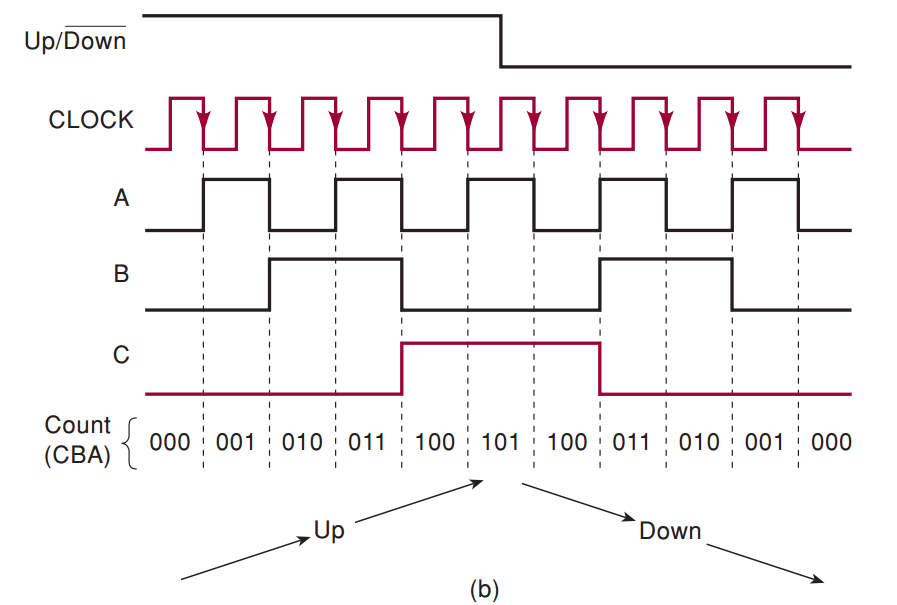
\includegraphics[scale = 0.6]{hinh48}
\bigbreak
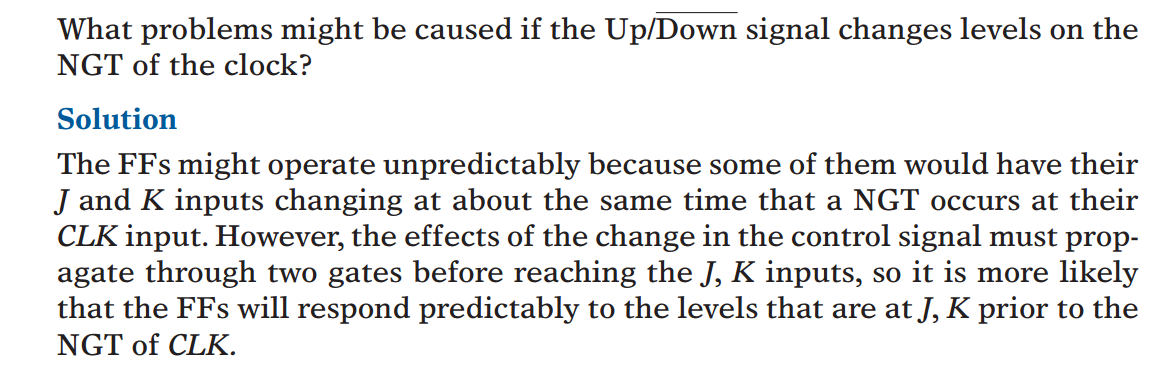
\includegraphics[scale = 0.6]{hinh49}
\bigbreak
\subsection{Presetable Counter}
- Presetable Counter is the counter that can be preset to any desired starting count either asynchronously or synchronously. \\
- This presetting operation is also reffered to as \textbf{parallel loading}. \\
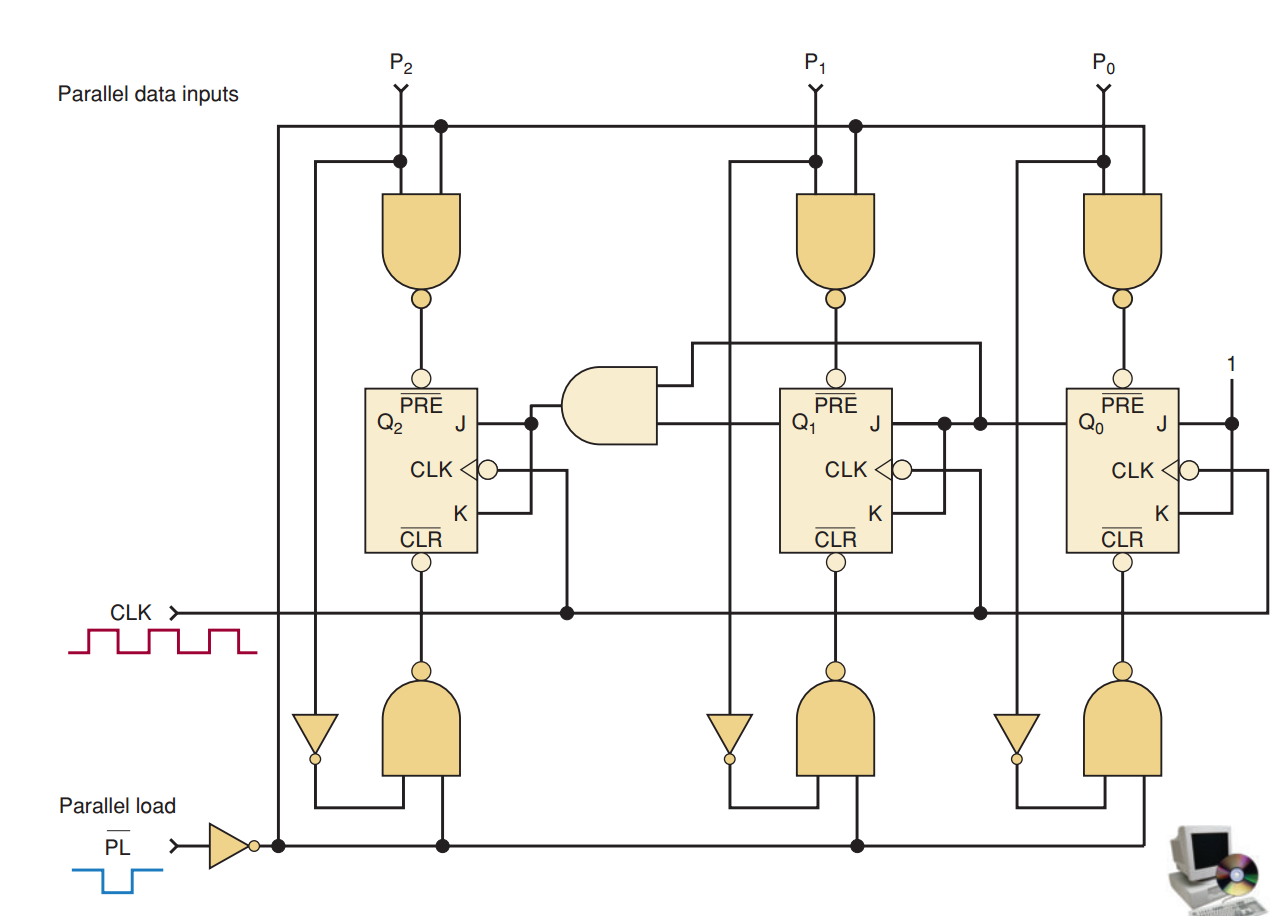
\includegraphics[scale = 0.6]{hinh50}
\bigbreak
\begin{itemize}
	\item Apply the desired count to the parallel data inputs ($P_{2}, P_{1}, P_{0}$).
	\item Apply a LOW pulse to the PARALLEL LOAD input, $\bar{PL}$
	\item This procedure will perform the asynchronous transfer to $P_{2}, P_{1}, P_{0}$ levels into flip-flops $P_{2}, P_{1}, P_{0}$. This \textbf{tram transfer} occurs independently of the J, K and CLK inputs.
	\item  The effect of the CLK input will be disabled when $\bar{PL}$ is LOW because each FF will have one of its asynchronous inputs activated while $\bar{PL}$ = 0.
	\item Once $\bar{PL}$ returns HIGH, the FFs can respond to their CLK inputs and can resume the counting-up operation.
	\item This asynchronous presetting is used by several IC counters ( the
TTL 74ALS190, 74ALS191, 74ALS192, and 74ALS193 and the CMOS equivalents, 74HC190, 74HC191, 74HC192, and 74HC193.)
\end{itemize}
\subsection{Synchronous Presetting}
- Many IC parallel counters use synchronous presetting whereby the counter is
preset on the active transition of the same clock signal that is used for counting.The logic level on the parallel load control input determines if the counter
is preset with the applied input data at the next active clock transition. \\
- Examples of IC counters that use synchronous presetting include the
TTL 74ALS160, 74ALS161, 74ALS162, and 74ALS163 and their CMOS equivalents, 74HC160, 74HC161, 74HC162, and 74HC163.\\
\subsection{IC Synchronous Counters}
\textbf{The 74ALS160-163 / 74HC160-163 Series} \\
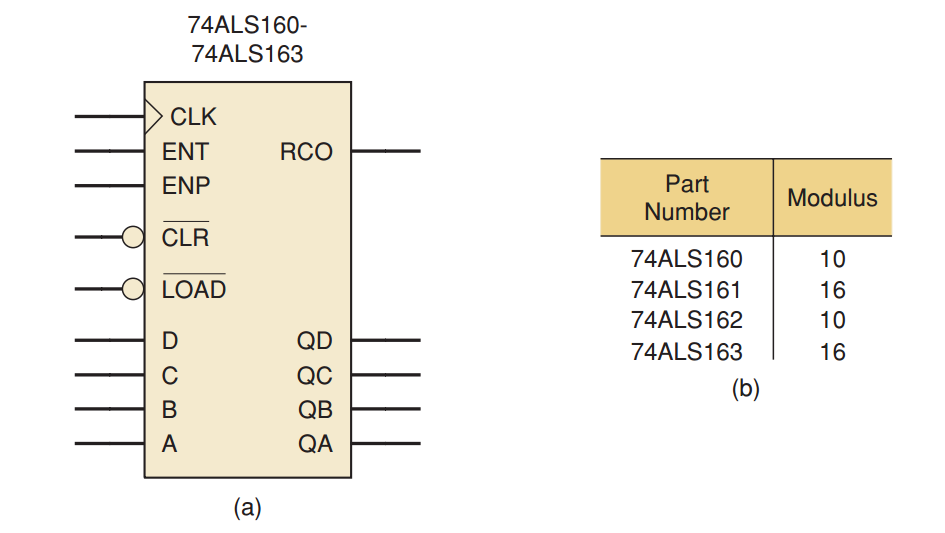
\includegraphics[scale = 0.7]{hinh51}
\bigbreak
\includegraphics[scale = 0.7]{hinh52}
\bigbreak
- In the 74ALS160-163 series:
\begin{itemize}
	\item Two of counters are the MOD-10 counters (74ALS160 and 74ALS162), while the other two is MOD-16 counter (74ALS161 and 74ALS163).
	\item The operation of the CLEAR function: \\
	- The 74ALS160 and 74ALS161 has asynchronous clear input. \\
	- THE 74ALS162 and 74ALS163 has synchronous clear input. \\
	\item About the parallel loading of data into the counter's FFs: \\
	- To preset a data value, make the CLEAR input inactive (HIGH), apply the desired four-bit value to the data input pins D, C, B, A (A is LSB and D is MSB), apply LOW to the $\bar{LOAD}$ input control, and the CLK with PGT. \\
	- The LOAD function is synchronous and has priority over counting, so it doesn't matter the what logic levels are applied to ENT or ENP. \\
	\item To enable counting, the CLEAR and LOAD musu be at inactice states, ENT and ENP are both HIGH and if one of them are LOW then the counter will hold the current state (no change). \\
	\item When counting, the decade counters (74ALS160 and 74ALS162) will automatically recycle to 0000 after state 1001 (9) and the binary counters (74ALS161 and 74ALS163) will automatically recycle after 1111 (15).
	\item This series of IC counter chips has one more output pin, RCO. This function of active-HIGH output is to detect (decode) the last state of the counter. \\
	- ENT must be HIGH for the counter to indicate with the RCO output that it has reached its terminal state.
\end{itemize}
\bigbreak
\textbf{THe 74ALS190-191 / 74HC190-191 Series} \\
\includegraphics[scale = 0.5]{hinh53}
\bigbreak
\subsection{Multistage Arrangment}
\includegraphics[scale = 0.6]{hinh54}
- The procedure of the Multistage Arrangment: \\
\begin{itemize}
	\item EN, the enable for the eight-bit counter, is connected to ENT output on stage 1 since ENT control the RCO output.
	\item Both counter blocks are clocked together synchronously, but the block on the stage 2 is disabled until the last-significant output has reached its terminal stage, incicated as TC1.
	\item When Q3, Q2, Q1, reaches 1111 and if EN is HIGH, then TC1 will output a HIGH. This will allow both counter stages to count up one with the next PGT on the clock.
	\item Stage 1 will back to 0000 and stage 2 will increment from its previous output state. TC1 is LOW and stage 1 is no longer to at it terminal stage.
\end{itemize}
\subsection{Decoding the Counter}
- Decode is the conversion of the binary output to a decimal value. \\
\begin{enumerate}
	%1
	\item \textbf{ACTIVE-HIGH Decoding: } \\
	- A active-HIGH decoding produces HIGH outputs to indicate detection. \\
	\includegraphics[scale = 0.7]{hinh55}
	\bigbreak
	\includegraphics[scale = 0.5]{hinh56}
	\bigbreak
	- The decoder consists of eight three-bit input AND gates. Each AND gate produces a HIGH output for one particular state of the counter. \\
	%2
	\item \textbf{ACTIVE-LOW Decoding: } \\
	- If we replace AND gates by NAND gates, the decoder outputs produce a normal HIGH signal, which goes LOW only when the number being decoded occurs. \\
\end{enumerate}
\subsection{BCD Counter Decoding}
- A BCD counter has 10 states that can be decoded and provides 10 outputs corresponding to the decimal digits 0 thorough 9 and represented by the states of the counter FFs. \\
\includegraphics[scale = 0.8]{hinh60}
\bigbreak
- These 10 outputs can be used to control invidual indicator LEDs for a visual display and use a single display device instead of 10 separate LEDS to display the decimal number from 0 to 9. \\
\includegraphics[scale = 0.7]{hinh61}
\bigbreak

\subsection{Analyzing Synchronous Counter:}
- To analyze the Synchronous Counter we use a \textbf{PRESENT/NEXT} stage table: \\
 \begin{itemize}
     \item Write the logic expression for each Ff control input.
     \item Assume the \textbf{PRESENT} state for the counter and apply the combination of bits to the control logic  expressions. The outputs from the control expression will allow us to predict \textbf{NEXT} for the counter after clocking.
 \end{itemize}
 \bigbreak
\subsection{Synchronous Counter Design:}
\begin{enumerate}
    \item J-K Excitation Table: \\
    \includegraphics[scale = 0.7]{hinh62}
    \bigbreak
    \item D Exitation Table: \\
    - For D FF D will have the value of the \textbf{NEXT} stage: \\
    \begin{tabular}{|c|c|c|}
    \hline
    PRESENT & NEXT & D \\
    \hline
     0 & 0 & 0 \\
     \hline
     0 & 1 & 1 \\
     \hline
     1 & 0 & 0 \\
     \hline
    \end{tabular}
\end{enumerate}

\section{MSI (Medium Scale Itegration) Logic Circuit}
\subsection{Decoders}
- A \textbf{Decoder} is a logic circuit that accepts a set of inputs that represents a binary number and activates only the outputs that corresponds to that input number. \\
- A \textbf{decoder circuit} looks at the inputs, determines which binary number represent there, and activates the outputs of that number, the other outputs will remain inactive. \\
\includegraphics[scale = 0.7]{hinh57}
\bigbreak
- In the picture: \\
\begin{itemize}
 \item there are N-inputs can be 0 or 1 so that there are $2^{N}$ inputs combination or codes.
 \item For each of these input combinations, only one of the M outputs will be stay HIGH; all the other outputs will stay LOW.
 \item Many decoder are designed to produce te active-LOW outputs while all the other will stay HIGH.
 \item Not all the decoders ultilize all of $2^{N}$ possible inputs but only the certai n ones.
\end{itemize}

\textbf{ENABLE Input} \\
- Some decoders have one or more than ENABLE inputs that are used to control the operation of the decoder. \\
- With the ENABLE line is HIGH, the decoder will function normally and the A, B, C will determine which output is HIGH. \\
- When the ENABLE line is LOW, \textbf{all} of the output will be forced to the LOW state regardless of the levels at the A, B, C inputs. \\
\bigbreak
\textbf{3-Line to 8-Line Decoder: } \\
\includegraphics[scale = 0.6]{hinh75}
\bigbreak
\includegraphics[scale = 0.6]{hinh77}
\bigbreak
\textbf{74ALS138 1-of-8 Decoder: } \\
\includegraphics[scale = 0.6]{hinh78}
\bigbreak
\begin{itemize}
	\item The input code is applied at $A_{2}$, $A_{1}$ and $A_{0}$, where $A_{2}$ is the MSB.
	\item Inputs $\bar{E_{1}}$, $\bar{E_{2}}$ and $E_{3}$ are separately enable inputs that are combined in AND gate. 
	\item To enable the output NAND gates to respond to the input code at $A_{2} A_{1} A_{0}$ this AND gate must be HIGH.
\end{itemize}
\bigbreak
\textbf{BCD-to-Decimal Decoder: } \\
\includegraphics[scale = 0.6]{hinh79}
\bigbreak
\includegraphics[scale = 0.5]{hinh80}
\bigbreak 

\textbf{Decoder Application} \\
- Decoders are used whenever an output or group of the outputs is to be activated only on the occurence of a specified combination. \\
- These input levels are often provided by the outputs of a counter or a register. When the decoder inputs are connected with a counter that is being continually pulsed, the decoder outputs will be activated sequentially and they can be used as timing or sequencing signals to turn devices on or off at specific time. \\
- Decoder are wirely used in the memory system where they respond to the address code generated by the general processor to activated the particular memory location: \\
\begin{itemize}
	\item Each memory IC consists of many register that can store binary numbers (data).
	\item Each register has it own unique address to distinguish with the other register.
	\item A decoder is built into the memory IC's circuitry and allows a particular storage register to be activated when the combination of inputs are activated.
\end{itemize}
\subsection{Encoder}
- Most decoders accept an input code and produce a HIGH (or LOW) at one output line. The opposite of decode process is \textbf{encoding} and is performed by a logic circuit called an \textbf{encoder}. \\
- An encoder has a number of input lines, only one of which is activated at a given time and produces an N-bit output code, depending on which input is activated. \\
\includegraphics[scale = 0.7]{hinh58}
\bigbreak
\includegraphics[scale = 0.6]{hinh59}
\bigbreak
- A LOW at any single input will produce the output binary code corresponding to that input. \\
- $A_{0}$ is not connected to the logic gates because the encoder outputs will normally be at 000. \\
\subsection{Prority Encoder}
- One drawback of the simple encoder is when more than one input are activated at one time. \\
- So we will have a necessary logic gate to ensure that when we have more than one inputs, the output will correspond to the highest-numbered input. \\
\subsection{74147 Decimal to BCD Priority Encoder}
(sẽ thêm vào sau)
\subsection{Switch Encoder}
- The switch acts as open type, when a digit is depressed the circuit will produce the BCD code for that digit. \\
- The switch is used whenever the BCD data must be entered manually to the digital system. \\
- When the first key is depressed, the BCD code for that digits is sent to a four-bit FF register, when the second key depressed, the BCD code for that digits is sent to \textbf{another} four-bit FF register. \\
- Each four-bit register drives a decoder/driver and a numerial number display so that the number can be displayed. \\



\subsection{Multiplexer (Data Collector)}
- A digital multiplexer or data selector is a logic circuit that accepts several digital data inputs and selects one of them at any given time to pass on to the output. \\
- The routing of the desired data input to the output is controlled by SELECT inputs: \\
- The multiplexer acts like  a digitally contrlled multiposition switch where the digital code appied to the SELECT input controls which data inputs is switched into the output. \\
\includegraphics[scale = 0.7]{hinh63}
\bigbreak
\textbf{Two-Input Multiplexer} \\
- For a two-input multiplexer with data inputs $I_{0}$ and $I_1$ and the SELECT input. \\
\includegraphics[scale = 0.6]{hinh64}
\bigbreak
- The boolean expression for the output Z is: \\
\begin{center}
    $Z = I_{0} \bar{S} + I_{1} S$
\end{center}
- When S = 0, this expression becomes: \\
\begin{align}
    Z &= I_{0} \cdot 1 + I_{1} \cdot 0 \\
    &= I_{0}
\end{align}
\bigbreak
\textbf{4-input Multiplexer} \\
\includegraphics[scale = 0.6]{hinh65}
\bigbreak
\textbf{8-input Multiplexer} \\
\includegraphics[scale = 0.6]{hinh66}
\bigbreak
\includegraphics[scale = 0.6]{hinh67}
\bigbreak

\subsection{Quad 2-Input MUX} (74ALS157)
\includegraphics[scale = 0.6]{hinh68}
\bigbreak
\includegraphics[scale = 0.6]{hinh69}
\bigbreak

\subsection{MUX Application}
\textbf{Data Routing} \\
- Multiplexer can route data from one of several sources to one destination. The circuit below shows the system for displaying two multidigit BCD counters and choose to display one LED only at time. \\
\includegraphics[scale = 0.7]{hinh70}
\bigbreak
\begin{enumerate}
    \item Each counter consists of either 2 BCD counters and each one is driven by its own CLK.
    \item When the \textbf{COUNTER SELECT} line is HIGH, the ouputs of counter 1 will be will be allowed to pass through the multiplexer to the decoder (7447) and display on lED. When the \textbf{COUNTER SELECT} = 0, the output of counter 2 will be allowed to pass through the multiplexer to the decoder and display on LED.
\end{enumerate}
\bigbreak
\textbf{Parallel to Serial Conversion} \\
\includegraphics[scale = 0.6]{hinh71}
\bigbreak
- The data is present in parallel form at the outputs of X register and are fed to the 8-input MUX. \\
- A 3-bit MOD3 counter is used to provide the select code bits $S_{2} S_{1} S_{0}$
 so they cycle through from 000 to 111 as CLK pulses are applied. \\
 Ex: We have the signal where $X_{7} X_{6} X_{5} X_{4} X_{3} X_{2} X_{1} X_{0}$ = 10110101. \\
 \textbf{Solution:} This conversion process takes a total 8-CLK cycles. Note that $X_{0}$ is the LSB and $X_{7}$ is MSB. \\
 \bigbreak
 \subsection{Demultiplexer (Data Distributor:)}
 - A demultiplexer does reversed operation to the multiplexer: it takes a single input and distributes several outputs. \\
 \includegraphics[scale = 0.6]{hinh72}
 \bigbreak
 - In demultiplexer, the select input code determines to which output the DATA input will be transmitted. \\
 - In other words, the demultiplexer takes ont input data source and selectively distributes it to 1 of N output channels just like a multiposition switch. \\
 \bigbreak
 \textbf{1-Line to 8-Line Demultiplexer: } \\
 \includegraphics[scale = 0.5]{hinh73}
 \bigbreak
 - The single data input line I is connected to all 8 AND gates, but only one of these gates will be enabled by the SELECT input lines. For each SELECT code the demultiplexer will decides which output will be distributed. \\
 \includegraphics[scale = 0.6]{hinh74}
 \bigbreak
















\section{Fuzzy Logic}
- Fuzzy Logic (FL) is a method of reasoning that resemble the human reasoning.\\
- Unlike Combinational Logic which only takes precise input and produce a definite output as 0 and 1. \\
- Fuzzy Logic provide the wide range of the output that surround the value of 0 and 1.\\
\begin{itemize}
	\item To simlify the the result is 1, we can give the output of around 0.75 or 0.9 when the result is 0, the output can be a 0.34 or 0.2.
	\item The Fuzzy Logic works on the levels of possiblities of inputs to achieve the definite output.
	\item Fuzzy Logic is useful for commercial and practical product. \\
	- It can control machines and consumer products. \\
	- It may not give a accurate result, but it still a acceptable result. \\
	- Fuzzy logic help to deal with the uncertainly in engineering.
\end{itemize}
\subsection{Fuzzy logic system}
- It has 4 main parts: \\
\begin{itemize}
	\item Fuzzification Module: \\
	- It transforms the system inputs, from  crisp number to fuzzy set. \\
	- Crisp number is a single point, ex: 3, 5.5, 6; when fuzzy number is a fuzzy set with different degree os closeness to a given crisp number. \\
	- It splits the input signal into 5 components: \\
	\begin{tabular}{|c|c|}
	\hline
	LP & x is Large Positive \\
	\hline
	MP & x is Medium Positive \\
	\hline
	S & x is small \\
	\hline
	MN & x is Medium Negative \\
	\hline
	LN & x is Large Negative \\
	\hline
	\end{tabular}
	\bigbreak
	\item Knowledge Base: \\
	- It stores IF-THEN rules.
	\item Inference Engine: \\
	- it simulates the human reasoning process by making fuzzy inference on the inputs and IF-THEN.
	\item Defuzzification Module: \\
	- It transforms the fuzzy set obtained by the inference engine into crisp value.
\end{itemize}
\includegraphics[scale = 0.6]{hinh16}
\bigbreak
\section{Half Adder and Full Adder}
- In digital system, an adder is a \textbf{digital circuit} in electronics that implies the addition of numbers. \\
- It is used in the arithmetic logic units.
- It also untilizes the many parts of the processors, address, ... etc. \\
\subsection{Half Adder}
\begin{itemize}
	\item The half adder adds 2 binary inputs and produce the 2 outputs as SUM and CARRY; XOR gate is applied to both inputs to produce SUM; when AND gate is applied to produce CARRY.
	\item \includegraphics[scale = 0.6]{hinh17}
	\item \includegraphics[scale = 0.6]{hinh18}
\end{itemize}
\subsection{Full Adder}
\begin{itemize}
	\item The different between Full Adder and Half Adder is Full Adder use 3 binary inputs, which 2 of inputs can be reffered as operands and the other one is a bit carried in.
\end{itemize}
\end{document}
